\documentclass[12pt,a4paper,oneside]{report}

% =========================================================
% VESIT MAJOR PROJECT REPORT TEMPLATE
% Academic Year: 2026--2027
%
% IMPORTANT:
% 1. Replace the logo files in figures/ when available.
% 2. Edit project_details.tex for student/project details.
% 3. Write the report chapter-wise inside chapters/.
% =========================================================

\usepackage[utf8]{inputenc}
\usepackage[T1]{fontenc}
\usepackage{graphicx}
\usepackage{amsmath,amssymb}
\usepackage{booktabs}
\usepackage{array}
\usepackage{longtable}
\usepackage{multirow}
\usepackage{float}
\usepackage{caption}
\usepackage{subcaption}
\usepackage{setspace}
\usepackage{geometry}
\usepackage{fancyhdr}
\usepackage{titlesec}
\usepackage{enumitem}
\usepackage{xcolor}
\usepackage{url}
\usepackage[hidelinks]{hyperref}
\usepackage{cite}
\usepackage{listings}
\usepackage{tikz}
\usepackage{etoolbox}
\usepackage{pdflscape}

% ---------------------------------------------------------
% Page setup
% ---------------------------------------------------------
\geometry{
    a4paper,
    left=1.5in,
    right=1in,
    top=1in,
    bottom=1in
}

\setstretch{1.18}
\setcounter{tocdepth}{1}
\setlength{\parindent}{0.5in}
\setlength{\parskip}{0pt}
\setlength{\emergencystretch}{3em}

% ---------------------------------------------------------
% Project details and logo configuration
% ---------------------------------------------------------
% =========================================================
% PROJECT DETAILS
% Edit ONLY this file for basic project information.
% =========================================================

% ---------- Institute ----------
\newcommand{\institutename}{VESIT}

\newcommand{\fullinstitutename}{Vivekanand Education Society's Institute of Technology}

\newcommand{\instituteaffiliation}{An Autonomous Institute Affiliated to University of Mumbai}

\newcommand{\instituteaddress}{Hashu Advani Memorial Complex, Collector Colony, Chembur East, Mumbai - 400074}

\newcommand{\departmentname}{Department of Artificial Intelligence and Data Science}
\newcommand{\shortdepartment}{Department of AI\&DS}

% ---------- Project ----------
\newcommand{\projecttitle}{Death by a Thousand Cuts: Mapping the Breaking Point of Machine Learning Models Under Compound Noise}
\newcommand{\projectsubtitle}{A Mini Project Report}

% ---------- Students ----------
\newcommand{\studentone}{Rushikesh Tathe}
\newcommand{\studentoneprn}{Roll No: 54}

\newcommand{\studenttwo}{Nihar Gudekar}
\newcommand{\studenttwoprn}{Roll No: 64}

\newcommand{\studentthree}{Mohammad Ali Sayyed}
\newcommand{\studentthreeprn}{Roll No: 65}

\newcommand{\studentfour}{Student Name}
\newcommand{\studentfourprn}{PRN / Roll No.}

% ---------- Faculty ----------
% Project Guide
\newcommand{\guidename}{Mrs. Bincy Ivin}
\newcommand{\guideDesignation}{Subject Teacher}

% Head of Department
\newcommand{\hodname}{Dr. Anjali Yeole}
\newcommand{\hodDesignation}{Head of Department}

% Principal
\newcommand{\principalname}{Dr. JM Nair}
\newcommand{\principalDesignation}{Principal}

% ---------- Academic year ----------
\newcommand{\academicYear}{2026--2027}

% ---------- Logo locations ----------
% Put the actual image files in the figures/ folder.
\newcommand{\vesitlogo}{figures/VESIT LOGO ICON (1).png}
\newcommand{\universitylogo}{figures/university_logo.png}

% ---------- Header text ----------
% Change these later if VESIT provides a prescribed format.
\newcommand{\leftheader}{\shortdepartment}
\newcommand{\rightheader}{MINI Project-II Report}


% =========================================================
% HEADER AND FOOTER
% =========================================================

\pagestyle{fancy}
\fancyhf{}

% Header
\fancyhead[L]{\small\bfseries \leftheader}
\fancyhead[R]{\small\bfseries Mini Project \nouppercase{\leftmark}}

% Header line
\renewcommand{\headrulewidth}{0.4pt}

% Footer
\fancyfoot[C]{\thepage}

% Footer line
\renewcommand{\footrulewidth}{0pt}

% Header/footer spacing
\setlength{\headheight}{15pt}
% Make chapter-opening pages use the same header/footer
\fancypagestyle{plain}{
    \fancyhf{}
    \fancyhead[L]{\small\bfseries \leftheader}
    \fancyhead[R]{\small\bfseries Mini Project \nouppercase{\leftmark}}
    \fancyfoot[C]{\thepage}
    \renewcommand{\headrulewidth}{0.4pt}
    \renewcommand{\footrulewidth}{0pt}
}

% ---------------------------------------------------------
% Chapter formatting
% ---------------------------------------------------------
\titleformat{\chapter}[display]
  {\normalfont\bfseries\centering}
  {\chaptername\ \thechapter}
  {10pt}
  {\Large}

\titlespacing*{\chapter}{0pt}{-10pt}{25pt}

% ---------------------------------------------------------
% Captions
% ---------------------------------------------------------
\captionsetup{
    font=small,
    labelfont=bf,
    justification=centering
}

% ---------------------------------------------------------
% Code listing style
% ---------------------------------------------------------
\lstset{
    basicstyle=\ttfamily\small,
    breaklines=true,
    frame=single,
    numbers=left,
    numberstyle=\tiny,
    showstringspaces=false
}

% ---------------------------------------------------------
% Helper command for optional images
% ---------------------------------------------------------
\newcommand{\insertlogo}[2][3cm]{%
    \IfFileExists{#2}{%
        \includegraphics[width=#1]{#2}%
    }{%
        \fbox{\parbox[c][2cm][c]{3cm}{\centering Logo\\Placeholder}}%
    }%
}

\begin{document}

% =========================================================
% FRONT MATTER
% =========================================================
\pagenumbering{roman}

\begin{titlepage}
\thispagestyle{empty}

\begin{center}

\vspace*{0.2cm}

% =========================================================
% INSTITUTE
% =========================================================

{\LARGE\bfseries \fullinstitutename\par}

\vspace{0.5cm}

{\small \instituteaffiliation\par}

\vspace{0.05cm}

{\small \instituteaddress\par}

\vspace{0.4cm}

% =========================================================
% DEPARTMENT
% =========================================================

{\Large\bfseries \departmentname\par}

\vspace{0.5cm}

% =========================================================
% LOGO
% =========================================================

\includegraphics[width=3cm]{\vesitlogo}

\vspace{0.9cm}

% =========================================================
% PROJECT TITLE
% =========================================================

{\large A Mini Project Report on\par}

\vspace{0.2cm}

{\LARGE\bfseries \projecttitle\par}

\vspace{0.9cm}



% =========================================================
% STUDENTS
% =========================================================

{\normalsize\bfseries Submitted by\par}

\vspace{0.15cm}

\begin{tabular}{ll}
\studentone   & \studentoneprn\\
\studenttwo   & \studenttwoprn\\
\studentthree & \studentthreeprn\\
\end{tabular}

\vspace{0.9cm}

% =========================================================
% GUIDE
% =========================================================

{\normalsize\bfseries Under the Guidance of\par}

\vspace{0.5cm}

{\large \guidename\par}

\vfill

% =========================================================
% ACADEMIC YEAR
% =========================================================

{\large\bfseries Academic Year \academicYear\par}

\vspace{0.2cm}

\end{center}

\end{titlepage}
\chapter*{Certificate}
\addcontentsline{toc}{chapter}{Certificate}

This is to certify that the project entitled \textbf{``\projecttitle''} has been carried out by \textbf{\studentone}, \textbf{\studenttwo}, and \textbf{\studentthree} under the guidance of \textbf{\guidename} in partial fulfillment of the requirements for the award of the degree of Bachelor of Engineering in Artificial Intelligence and Data Science during the academic year \academicYear.

\vspace{5cm}

\begin{center}

\begin{tabular}{p{4.4cm} p{4.4cm} p{4.4cm}}

\textbf{\guidename} &
\textbf{\hodname} &
\textbf{\principalname} \\[1.0cm]

\guideDesignation &
\hodDesignation &
\principalDesignation

\end{tabular}

\end{center}

\vfill

\noindent Date: \rule{4cm}{0.4pt}
\hfill
Place: Mumbai

\chapter*{Declaration}
\addcontentsline{toc}{chapter}{Declaration}

We hereby declare that the project entitled \textbf{``\projecttitle''} is our original work carried out under the guidance of \textbf{\guidename}. The work presented in this report has not been submitted elsewhere for the award of any degree or diploma, except where due acknowledgement has been made.

\vspace{1.5cm}

\begin{tabular}{p{0.45\textwidth} p{0.45\textwidth}}
\textbf{Name} & \textbf{Signature}\\[0.8cm]
\studentone & \rule{4cm}{0.4pt}\\[0.5cm]
\studenttwo & \rule{4cm}{0.4pt}\\[0.5cm]
\studentthree & \rule{4cm}{0.4pt}
\end{tabular}

\chapter*{Acknowledgement}
\addcontentsline{toc}{chapter}{Acknowledgement}

We would like to express our sincere gratitude to our project guide, \guidename, for her constant guidance, constructive feedback, and encouragement throughout the planning and development of this mini project. Her suggestions helped us sharpen the research question and maintain a rigorous experimental methodology.

We are thankful to the Head of the Department and the faculty members of the \departmentname\ for providing the academic environment and resources needed to complete this work. We also acknowledge the support of the institute in providing access to the scholarly databases used for the literature review.

We thank our colleagues, friends, and family for their encouragement and support.

\vspace{1cm}

\begin{flushright}
\begin{tabular}{r}
\studentone\\
\studenttwo\\
\studentthree
\end{tabular}
\end{flushright}

\chapter*{Abstract}
\addcontentsline{toc}{chapter}{Abstract}

Real-world training data can contain incorrect labels, noisy features, outliers and missing values. This project investigates how these corruptions, individually and in combination, affect classical machine learning models on tabular data.

A reproducible experimental framework evaluates Logistic Regression, RBF Support Vector Machine, Decision Tree and Random Forest on the Breast Cancer and Digits datasets. All fifteen non-empty combinations of four noise types are tested at five severity levels, using ten seeds and a stratified 70/30 split. The 6,080 fits apply noise only to training data and evaluate on a clean test set. Macro F1 is the primary metric and accuracy is secondary. A model's breaking point is the first level at which its mean Macro F1 falls to 90\% or less of its clean baseline. The Breaking Point Index and Robustness Score summarise performance, while a synergy analysis compares compound and individual noise effects.

In the official benchmark, label noise is the most damaging single corruption. Mean breaking levels fall from 5.281 for single noises to 3.750 for the four-way combination, counting a threshold not reached as level 6. Decision Tree is least robust on both datasets, while Random Forest has the highest mean Breaking Point Index and Logistic Regression retains the highest mean share of its clean Macro F1.

A separate demonstration uses all 581,012 records from UCI Covertype, a real-world forest-cover classification dataset. Across 16 Decision Tree fits using one seed, clean Macro F1 is 0.8950. The breaking point is level 1 for label noise and for label noise combined with missing values, and level 3 for missing values alone. A FastAPI service and React application support result exploration, a Covertype preset, and custom CSV uploads.


\tableofcontents
\listoffigures
\listoftables

% Uncomment if a list of abbreviations is required.
% \input{frontmatter/abbreviations}

% =========================================================
% MAIN CONTENT
% =========================================================
\clearpage
\pagenumbering{arabic}

\chapter{Introduction}

\section{Background}

Machine learning models are only as reliable as the data used to train them. In controlled benchmarks, training data is assumed to be clean, correctly labelled, and complete. In practice, data is collected from sensors, surveys, hospital records, web sources, and human annotators, and it frequently contains mislabelled samples, noisy measurements, missing entries, and extreme observations. A model that performs well on a curated dataset can therefore degrade sharply when it is deployed on data that contains the same imperfections.

The problem of learning from imperfect data has been studied for several decades. Surveys on label noise describe how incorrect labels arise, how they affect conventional classifiers, and which families of methods have been proposed to make training more robust \cite{frenay2014classification,song2023survey}. A central observation is that sufficiently flexible models can memorise corrupted labels and still fit the training set, which harms generalisation on unseen data \cite{zhang2021rethinking}. Deep neural networks are particularly susceptible to this effect, although the severity depends on the architecture, the amount of data, and the noise rate \cite{rolnick2017robust}. Robust loss functions, sample selection, loss correction, regularisation, and specialised architectures have all been proposed to reduce the damage caused by label noise \cite{natarajan2013learning,song2023survey}.

Feature-space corruption is a separate but related problem. Gaussian feature noise, outliers, and missing values alter the input distribution rather than the labels. Robust statistics provides classical tools for limiting the influence of outliers \cite{huber1964robust}, while missing-value imputation and feature scaling are standard preprocessing steps. Recent work has also shown that feature noise and label noise interact: adding Gaussian noise to features can, under some conditions, tighten a generalisation bound and improve robustness to label noise in deep networks \cite{zeng2025feature}. Hybrid and compound noise settings, in which several corruption types occur together, have been studied in multilabel learning \cite{zhang2020hybrid} and in semisupervised deep generative models \cite{chen2023compound}.

Despite this body of work, two gaps remain. First, most studies focus on a single corruption type, or on a small number of selected combinations, and they usually report performance at one or two noise rates. Second, the dominant experimental setting is deep learning on image or graph data, whereas many practical tabular problems in medicine, finance, and public administration are still solved with classical models such as logistic regression, support vector machines, decision trees, and random forests. Practitioners therefore lack a systematic, reproducible description of how classical models fail as several corruption types accumulate.

The title of this project, \emph{Death by a Thousand Cuts}, captures the intuition behind the study. A single small corruption may be harmless, but many small corruptions applied together can push a model past a critical point. The project asks where that critical point lies, how it depends on the model, the dataset, and the corruption type, and whether the combined effect is larger or smaller than the sum of the individual effects.

\section{Problem Statement}

Given two clean tabular datasets and four fixed classical classifiers, the project studies how model performance changes when training data is corrupted by individual and compound noise. Four noise types are considered: label noise, Gaussian feature noise, outliers, and missing values. Every non-empty subset of these four types is evaluated, giving fifteen noise combinations, and each combination is applied at five increasing severity levels. The test set is always clean and is never used for fitting or noise estimation.

Formally, let $D = \{(x_i, y_i)\}_{i=1}^{n}$ be a dataset, let $M$ be a classifier, and let $C \subseteq \{\text{label}, \text{Gaussian}, \text{outliers}, \text{missing}\}$ be a non-empty noise combination with $|C| \geq 1$. For a severity level $L \in \{1,\ldots,5\}$, let $D^{\text{train}}_{C,L}$ be the corrupted training split and let $D^{\text{test}}$ be the untouched clean test split. The experiment fits $M$ on $D^{\text{train}}_{C,L}$ and evaluates Macro F1 and Accuracy on $D^{\text{test}}$. The clean baseline $B_{M}$ is the mean Macro F1 of $M$ on $D^{\text{test}}$ when trained on the clean training split.

The breaking point of model $M$ for combination $C$ is the first level $L^{*} \in \{1,\ldots,5\}$ for which
\begin{equation}
  \overline{\text{F1}}_{M,C}(L^{*}) \;\leq\; 0.90 \times B_{M},
  \label{eq:breaking}
\end{equation}
where $\overline{\text{F1}}_{M,C}(L)$ is the mean Macro F1 over the official seeds. If no level satisfies the condition, the breaking point is reported as \emph{not reached}.

The project addresses the following research question and sub-questions:

\begin{itemize}
  \item \textbf{RQ.} How do individual and compound noise affect machine learning model robustness, and where does each model reach its breaking point?
  \item \textbf{Q1.} Which model is most robust overall?
  \item \textbf{Q2.} Which noise type causes the largest degradation?
  \item \textbf{Q3.} What is the breaking point of each model for each noise type and combination?
  \item \textbf{Q4.} Is compound noise worse than the sum of its single-noise components?
  \item \textbf{Q5.} Do the results differ between binary (Breast Cancer) and multiclass (Digits) data?
\end{itemize}

\section{Motivation}

Data quality is one of the most important determinants of model reliability. When a model fails in a medical, financial, or operational setting, the cause is often a change in the input distribution, a corrupted label, or a missing value rather than a deficiency of the learning algorithm. Understanding which corruption type is most damaging, and how much of it a model can tolerate, helps practitioners prioritise data-cleaning effort and choose models that are appropriate for noisy environments.

The existing literature provides strong evidence that label noise harms generalisation and that many mitigation methods can help \cite{song2023survey}. It also shows that feature noise can interact with label noise in non-obvious ways \cite{zeng2025feature}, and that compound noise is a recognised challenge in multilabel and semisupervised settings \cite{zhang2020hybrid,chen2023compound}. However, these studies do not provide a common protocol that sweeps all combinations of noise types over several severity levels, and they rarely report the point at which a classical model becomes unusable.

A second motivation is reproducibility. Robustness claims are difficult to compare when datasets, splits, noise models, model hyperparameters, and evaluation metrics differ across papers. This project addresses that problem by fixing the methodology before the main experiment, recording a configuration hash, freezing the severity table, storing per-fit provenance, and locking the final result artefacts with checksums. The resulting benchmark is small enough to run on a standard workstation but detailed enough to support quantitative analysis.

Finally, the project is motivated by the needs of teaching and applied research. A transparent, reproducible benchmark of classical models on tabular data is useful for students and practitioners who want to understand robustness without the computational cost and opacity of large deep networks.

\section{Objectives}

The objectives of the proposed project are:

\begin{enumerate}
  \item To design and implement a reproducible experiment engine that loads the two approved datasets, creates stratified training and test splits, injects four types of noise with deterministic random-number generation, and evaluates four fixed classical classifiers.
  \item To evaluate all fifteen non-empty combinations of label noise, Gaussian feature noise, outliers, and missing values at five severity levels, using a clean test set and a fixed preprocessing pipeline.
  \item To define and compute the breaking point of each model for each noise combination, together with two aggregate robustness measures: the Breaking Point Index (BPI) and the Robustness Score (RS).
  \item To perform a secondary synergy analysis that compares the observed compound-noise degradation with the sum of the corresponding single-noise degradations.
  \item To answer the research sub-questions Q1--Q5 using the frozen official results and to compare the findings with the published literature.
  \item To provide a read-only results API, an interactive React application for exploring the results, and a provenance and checksum mechanism that makes the official experiment auditable.
\end{enumerate}

\section{Scope}

The scope of the project is deliberately bounded so that the methodology remains reproducible and the results remain interpretable.

\textbf{In scope:}
\begin{itemize}
  \item Two public tabular datasets: Breast Cancer (569 samples, 30 features, 2 classes) and Digits (1,797 samples, 64 features, 10 classes).
  \item Four classical classifiers: Logistic Regression, SVM with an RBF kernel, Decision Tree, and Random Forest.
  \item Four noise types: label noise, Gaussian feature noise, outliers, and missing values.
  \item All fifteen non-empty noise combinations and five severity levels (1--5), with a clean level 0 baseline.
  \item A stratified 70/30 split, noise applied only to training data, and a clean test set.
  \item Macro F1 as the primary metric and Accuracy as the secondary metric.
  \item Breaking-point, BPI, RS, and synergy analyses.
  \item A Python experiment engine, a FastAPI service, a React visualization application, and file-based provenance.
\end{itemize}

\textbf{Out of scope:}
\begin{itemize}
  \item Deep learning models and neural architectures.
  \item Additional datasets, additional noise types, and real-world (instance-dependent) label noise.
  \item Hyperparameter tuning and model selection.
  \item Noise mitigation methods such as robust losses, sample selection, or cleaning.
  \item Class-imbalance experiments and irrelevant-feature noise.
  \item Authentication, cloud deployment, database storage, and distributed job queues.
\end{itemize}

\section{Contributions}

The main contributions of the project are as follows.

\begin{enumerate}
  \item \textbf{A systematic compound-noise benchmark for classical tabular models.} The project evaluates all fifteen non-empty combinations of four noise types at five severity levels, across four models and two datasets, using a fixed and documented protocol. The official run contains 6,080 fits over ten seeds.
  \item \textbf{A breaking-point formulation.} Instead of reporting only average accuracy, the project defines the breaking point as the first severity level at which mean Macro F1 falls to 90\% or less of the clean baseline. This makes the notion of ``model failure'' explicit and comparable across models and noise combinations.
  \item \textbf{Two aggregate robustness measures.} The Breaking Point Index summarises how long a model survives across combinations, and the Robustness Score summarises retained performance across levels. Ranking by BPI and then RS gives a concise model comparison.
  \item \textbf{A synergy analysis for compound noise.} The project measures whether the compound-noise drop is larger or smaller than the sum of the corresponding single-noise drops, and flags floor effects when the sum of single drops reaches the baseline.
  \item \textbf{A reproducible and auditable implementation.} The engine uses deterministic seed sequences, a frozen severity table, a configuration hash, per-fit provenance, manifests, and SHA-256 checksums. The official Full results are locked and immutable after verification.
  \item \textbf{Empirical findings.} The frozen results show that label noise is the most damaging single corruption, that compound noise is consistently more harmful than individual noise, that the multiclass dataset is more fragile than the binary dataset, and that the Decision Tree is the least robust model while Random Forest and Logistic Regression lead on different aggregate measures.
  \item \textbf{An interactive results application.} A FastAPI backend and a React frontend expose the official results through curves, heatmaps, breaking-point tables, robustness rankings, and a separate custom-experiment workflow.
\end{enumerate}

\section{Organization of the Report}

The remainder of the report is organised as follows.

\begin{itemize}
  \item \textbf{Chapter 2} reviews the literature on label noise, feature noise, compound noise, classical robust learning, and evaluation practice. It compares the reviewed papers and identifies the research gap addressed by this project.
  \item \textbf{Chapter 3} describes the proposed methodology, including the datasets, noise injectors, severity levels, preprocessing pipeline, models, and evaluation metrics.
  \item \textbf{Chapter 4} presents the system design: architecture, workflow, use cases, data flow, storage design, and module responsibilities.
  \item \textbf{Chapter 5} describes the implementation of the experiment engine, API, worker, and frontend, together with the security and privacy considerations.
  \item \textbf{Chapter 6} reports the experimental setup and the frozen official results, answers Q1--Q5, compares the findings with the literature, and discusses threats to validity.
  \item \textbf{Chapter 7} concludes the report, states the limitations, and outlines future work.
  \item The appendix documents the project's software and data contributions and the Sustainable Development Goals addressed by the work.
\end{itemize}

\chapter{Literature Review}

\section{Introduction}

The literature review examines how the research community has studied data corruption and model robustness, with emphasis on work that is directly relevant to individual and compound noise. The purpose is threefold: to establish what is already known, to identify the experimental settings that have been used, and to isolate the gap that the present project addresses.

The review was conducted using the IEEE Xplore Digital Library as the primary source, supplemented by ScienceDirect, SpringerLink, and Google Scholar for cross-checking metadata and for foundational papers. The search terms included combinations of \emph{noisy labels}, \emph{feature noise}, \emph{label noise robustness}, \emph{compound noise}, \emph{hybrid noise}, \emph{data corruption}, \emph{outliers}, \emph{missing values}, and \emph{classification}. Papers were included when they (i) appeared in a peer-reviewed journal or conference, (ii) addressed supervised classification under corrupted training data, and (iii) reported an experimental evaluation. Priority was given to four recent IEEE papers that collectively cover label noise, feature noise, hybrid noise, and compound noise. Foundational surveys and dataset papers were added to support the methodology.

The review is organised as follows. Section~2.2 describes the main families of existing approaches. Section~2.3 reviews the four core papers and the supporting literature in detail. Section~2.4 identifies the research gap, and Section~2.5 summarises the findings.

\section{Existing Systems}
Research on noisy data includes robust loss functions, sample selection and correction methods for label noise, as well as augmentation and robust estimation for feature corruption \cite{song2023survey,frenay2014classification,huber1964robust}. Classical classifiers remain useful for tabular data but are often evaluated under different datasets and noise assumptions \cite{hastie2009elements}.

\section{Review of Research Papers}
\paragraph{Fr\'enay and Verleysen.}
The survey distinguishes label errors that occur independently of an example from errors that depend on its true class or features \cite{frenay2014classification}. The project's label injector models uniform label noise by selecting a prescribed number of training rows at random and assigning each selected row a uniformly chosen alternative class.

\paragraph{Song et al.}
The survey groups deep-learning methods for noisy labels into robust architectures, regularisation, robust losses, loss adjustment, and sample selection \cite{song2023survey}. The present study uses classical classifiers with fixed settings and evaluates how their clean-test performance changes as training labels are corrupted.

\paragraph{Zhang et al.}
The proposed multilabel method uses relationships between labels and regularisation to address feature and label noise jointly \cite{zhang2020hybrid}. This motivates testing both input and label corruption in the same training split. The project evaluates single-label classifiers under individual and combined corruptions, with one target class per row.

\paragraph{Zeng et al.}
The authors show that appropriately chosen feature noise can improve generalisation for some deep networks trained with noisy labels \cite{zeng2025feature}. This motivates comparing label noise alone, Gaussian noise alone, and their combination in the official benchmark. Synergy measures departure from the sum of the individual drops. Whether Gaussian noise improved performance under label noise is assessed by comparing the combined condition directly with label noise alone.

\paragraph{Chen.}
The study addresses noisy labels and outliers together with a semisupervised generative model \cite{chen2023compound}. The present project includes outliers and label flips among four controlled corruption types and measures the resulting failure thresholds of classical tabular classifiers.

\section{Research Gap}

The reviewed literature establishes several important facts. Label noise harms generalisation, and many methods have been proposed to mitigate it \cite{song2023survey}. Feature noise can interact with label noise in non-obvious ways and can even improve robustness under some conditions \cite{zeng2025feature}. Hybrid and compound noise are recognised as realistic and difficult settings \cite{zhang2020hybrid,chen2023compound}. Classical models remain widely used on tabular data, but they are not inherently robust to corrupted labels \cite{frenay2014classification,song2023survey}.

At the same time, the literature leaves several gaps that are relevant to applied tabular machine learning.

\begin{enumerate}
  \item \textbf{Deep-learning bias.} The most comprehensive robustness studies focus on deep neural networks and image or graph benchmarks. Classical models on tabular data are underrepresented, even though they are common in medical, financial, and administrative applications.
  \item \textbf{Single-corruption bias.} Most studies examine label noise alone or feature noise alone. Compound noise is studied in selected settings, but there is no common protocol that enumerates all subsets of corruption types.
  \item \textbf{Limited severity sweep.} Robustness is usually reported at one or two noise rates. This makes it difficult to identify the point at which a model stops being useful.
  \item \textbf{No standard breaking-point measure.} The literature reports average accuracy or F1, but it does not define a model-specific failure threshold that can be compared across noise combinations.
  \item \textbf{Inconsistent evaluation protocols.} Datasets, splits, architectures, noise models, and metrics differ across papers, which limits direct comparison.
  \item \textbf{Weak treatment of synergy.} The combined effect of multiple noise types is often assumed to be additive or is discussed qualitatively, without an explicit decomposition into single-noise and interaction components.
\end{enumerate}

To the best of our knowledge, the reviewed literature does not report a single reproducible protocol that (i) enumerates all fifteen non-empty combinations of label noise, Gaussian feature noise, outliers, and missing values, (ii) sweeps five severity levels, (iii) evaluates four classical tabular models on both a binary and a multiclass dataset, and (iv) reports breaking points, aggregate robustness measures, and an explicit synergy analysis. This is the gap addressed by the present project.

The project does not claim to propose a new mitigation algorithm. Its contribution is a measurement framework and an empirical map. The framework makes the following aspects explicit and auditable:

\begin{itemize}
  \item the exact noise injectors and their parameters;
  \item the order in which compound noise is applied;
  \item the split and seed protocol;
  \item the definition of the breaking point;
  \item the aggregate robustness measures;
  \item the decomposition of compound effects into single-noise and interaction components;
  \item the provenance of every result row and the checksums of the final artefacts.
\end{itemize}

This positioning is important. The literature already provides strong evidence that noise harms models and that mitigation is possible. What it does not provide, in a single comparable protocol, is a map of \emph{where} classical tabular models break under individual and compound corruption. That map is the contribution of this project.

\section{Summary}

This chapter reviewed the main families of work on noisy data and model robustness. Label-noise research provides a mature taxonomy of robust architectures, regularisation methods, robust losses, loss adjustment, and sample selection \cite{song2023survey}. Feature-noise research shows that input corruption can interact with label corruption and can even improve generalisation in deep networks \cite{zeng2025feature}. Hybrid and compound-noise research shows that multiple corruption types must be considered together \cite{zhang2020hybrid,chen2023compound}. Classical robust learning provides the statistical and algorithmic background for handling outliers and noisy labels \cite{frenay2014classification,huber1964robust}.

The review also identified a clear gap: there is no systematic, reproducible, breaking-point-oriented comparison of classical tabular models under all combinations of label noise, Gaussian feature noise, outliers, and missing values. The next chapter describes the methodology designed to fill that gap.

\chapter{Proposed Methodology}

\section{Overview}

The project is implemented as a reproducible experiment engine with two interfaces. The engine performs all data loading, noise injection, model fitting, evaluation, and analysis. A command-line interface runs the official experiments, and a FastAPI service with a React frontend exposes the official results and supports separate custom experiments.

The methodology is fixed before the main experiment and is stored in a machine-readable configuration. The central idea is to hold everything constant except the corruption being studied. For every dataset and seed, the same stratified split is reused for all models and all noise combinations. The test set is never corrupted and is never used for fitting. For levels 1--5, the preprocessing pipeline and the classifier are fitted only on the corrupted training split. A single clean baseline fit at level 0 provides the reference performance for each dataset and model.

The engine evaluates four noise types, all fifteen non-empty combinations of those types, and five severity levels. This produces a dense performance surface that can be summarised as curves, breaking points, heatmaps, robustness rankings, and synergy estimates.

\section{System Requirements}

\subsection{Software Requirements}

The experiment engine is implemented in Python and uses the scientific Python stack. The frontend is implemented in TypeScript with React. Table~\ref{tab:software} lists the principal software components and the versions recorded in the official run manifest.

\begin{table}[H]
\centering
\caption{Principal software components and versions used for the official run.}
\label{tab:software}
\small
\begin{tabular}{p{4.0cm}p{3.4cm}p{5.6cm}}
\toprule
\textbf{Component} & \textbf{Version} & \textbf{Role} \\
\midrule
Python & 3.11.9 & Experiment engine, scripts, and API \\
NumPy & 1.26.4 & Numerical arrays and deterministic random generation \\
pandas & 2.2.2 & Tabular data handling and CSV output \\
SciPy & 1.13.1 & Scientific utilities used by scikit-learn \\
scikit-learn & 1.5.2 & Datasets, preprocessing, models, and metrics \\
matplotlib & 3.9.2 & Report figures \\
FastAPI & 0.115.0 & Read-only results API \\
Uvicorn & 0.30.6 & ASGI server \\
Pydantic & 2.9.2 & Request and response schemas \\
pytest & 8.3.3 & Automated tests \\
React, Vite, TypeScript & Current stable & Frontend application \\
Tailwind CSS, shadcn/ui & Current stable & Styling and UI components \\
Recharts, TanStack Query & Current stable & Charts and server-state management \\
CSV and JSON files & -- & Result storage, manifests, and job state \\
\bottomrule
\end{tabular}
\end{table}

\subsection{Hardware Requirements}

The official Full experiment is a single-process workload and does not require a GPU. It completed 6,080 fits in 703.8 seconds on a standard Windows workstation, with a mean fit time of 0.1038 seconds and a maximum fit time of 1.1598 seconds. A machine with at least 8 GB of RAM and a modern multi-core CPU is sufficient. The frontend and API can run on the same machine.

\subsection{Storage Requirements}

Results are stored as CSV and JSON files. The official Full run produces one raw row per fit and five derived analysis files. The manifest records the configuration, package versions, split hashes, and provenance information. No database is required.

\section{Proposed Approach}

The methodology proceeds in the following steps.

\begin{enumerate}
  \item \textbf{Load the dataset.} The selected dataset is loaded from scikit-learn. The feature matrix $X$ and the label vector $y$ are kept unchanged; no feature engineering is performed.
  \item \textbf{Create a stratified split.} For each dataset and seed $s$, the data is split into 70\% training and 30\% test using stratification on the class label. The split is computed once per $(dataset, seed)$ and reused for every model and every noise setting.
  \item \textbf{Keep the test set clean.} The test features and labels are stored separately and are never modified. All noise injection and all preprocessing statistics are computed from the training split only.
  \item \textbf{Estimate clean statistics.} The per-column mean $\mu_j$ and standard deviation $\sigma_j$ of the clean training features are computed. They are used only to size Gaussian noise and outliers, and to create the approved level-0 baseline.
  \item \textbf{Fit the clean baseline.} For each $(dataset, model, seed)$, the pipeline is fitted once on the clean training split. The result is stored with combination \texttt{clean} and level 0. This row is reused analytically as level 0 for every noise combination.
  \item \textbf{Apply noise.} For each combination $C$ and level $L \in \{1,\ldots,5\}$, the selected noise types are applied to the training split in the fixed order label, Gaussian, outliers, missing. The same noise realisation is used for a single noise and for the corresponding component inside a compound combination.
  \item \textbf{Fit the pipeline.} A fresh pipeline is fitted on the corrupted training split. The pipeline consists of mean imputation, standardisation, and the classifier. No step is fitted on the test set.
  \item \textbf{Evaluate.} The fitted pipeline predicts the clean test set. Macro F1 and Accuracy are recorded, together with the fit time and summary statistics of the injected noise.
  \item \textbf{Aggregate.} For each $(dataset, model, combination, level)$, the mean and sample standard deviation over the official seeds are computed. The clean baseline and the 90\% threshold are derived from the level-0 rows.
  \item \textbf{Analyse.} Breaking points, BPI, RS, and synergy are computed from the aggregated results, and the derived tables and figures are written to the official results directory.
\end{enumerate}

The split sizes are 398 training and 171 test samples for Breast Cancer, and 1,257 training and 540 test samples for Digits. The difference follows from the stratified 70/30 split and the dataset sizes.

\section{Algorithms / Models}

\subsection{Classification Models}

Four classical classifiers are used with fixed hyperparameters. No hyperparameter tuning or model selection is performed, because tuning would introduce a result-dependent degree of freedom that could undermine the comparison. Table~\ref{tab:models} lists the configurations.

\begin{table}[H]
\centering
\caption{Fixed classifier configurations.}
\label{tab:models}
\small
\begin{tabular}{p{3.2cm}p{6.2cm}p{3.8cm}}
\toprule
\textbf{Model} & \textbf{Configuration} & \textbf{Family} \\
\midrule
Logistic Regression & \texttt{LogisticRegression(}\newline\texttt{max\_iter=1000,}\newline\texttt{random\_state=seed)} & Linear, probabilistic \\
SVM (RBF) & \texttt{SVC(kernel='rbf', C=1.0, gamma='scale')} & Kernel, maximum margin \\
Decision Tree & \texttt{DecisionTreeClassifier(}\newline\texttt{random\_state=seed)} & Recursive partitioning \\
Random Forest & \texttt{RandomForestClassifier(}\newline\texttt{n\_estimators=100,}\newline\texttt{random\_state=seed,}\newline\texttt{n\_jobs=1)} & Bagged ensemble \\
\bottomrule
\end{tabular}
\end{table}

Logistic regression models the class posterior through a linear decision function and is a standard baseline for tabular classification \cite{hastie2009elements}. The support vector machine with an RBF kernel constructs a non-linear maximum-margin boundary \cite{cortes1995support}. The decision tree recursively partitions the feature space and is highly interpretable but sensitive to small changes in the data \cite{quinlan1986induction}. The random forest averages many randomised trees and usually reduces variance \cite{breiman2001random}.

\subsection{Preprocessing Pipeline}

The pipeline is the same for every model:
\begin{center}
\texttt{SimpleImputer(strategy='mean', keep\_empty\_features=True)} \\
$\rightarrow$ \texttt{StandardScaler} \\
$\rightarrow$ \texttt{Classifier}
\end{center}

Mean imputation is required because missing values are injected. Standardisation is required because the models have different sensitivities to feature scale, and because Gaussian noise and outliers are sized in units of the clean training standard deviation. The imputer and the scaler are fitted on the training split that is passed to the pipeline; at noisy levels, this is the corrupted training split. This prevents information from the test set from leaking into preprocessing.

\subsection{Noise Injectors}

The four noise injectors are deterministic given the seed, the noise identifier, and the severity level. The random generator is
\begin{equation}
\text{rng} = \texttt{np.random.default\_rng}\big(\texttt{SeedSequence}([s, \, id, \, L])\big),
\label{eq:rng}
\end{equation}
where $s$ is the seed, $id$ is the noise identifier (label = 1, Gaussian = 2, outliers = 3, missing = 4), and $L$ is the level. This construction ensures that the same component noise realisation is used when the noise appears alone and when it appears inside a compound combination.

\paragraph{Label noise.} For a flip rate $r$, the number of flipped labels is
\begin{equation}
n_{\text{flip}} = \operatorname{round}(r \cdot n).
\end{equation}
Indices are selected without replacement, and each selected label is replaced by a different class drawn uniformly from the remaining classes. The operation is applied to the training labels only.

\paragraph{Gaussian feature noise.} For a scale factor $k$ and per-column clean training standard deviation $\sigma_j$,
\begin{equation}
x_{ij} \leftarrow x_{ij} + z_{ij}, \qquad z_{ij} \sim \mathcal{N}(0,1)\cdot (k\sigma_j).
\end{equation}
Columns with $\sigma_j = 0$ are left unchanged. The noise is added cell-wise, so the number of affected cells is recorded in the noise statistics.

\paragraph{Outliers.} Eligible cells are those in columns with $\sigma_j > 0$. For an outlier cell rate $r$, the number of modified cells is
\begin{equation}
n_{\text{outlier}} = \operatorname{round}(r \cdot n_{\text{eligible}}).
\end{equation}
Selected cells are set to $\mu_j + 5\sigma_j$ or $\mu_j - 5\sigma_j$, with the sign chosen at random. This creates extreme values without changing the underlying column distribution for the remaining cells.

\paragraph{Missing values.} For a missing cell rate $p$, each cell is masked independently:
\begin{equation}
m_{ij} \sim \operatorname{Bernoulli}(p), \qquad x_{ij} \leftarrow \text{NaN if } m_{ij}=1.
\end{equation}
Missing values are injected last, after label noise, Gaussian noise, and outliers, so that imputation is not applied to cells that are later replaced by outliers.

Table~\ref{tab:noise} summarises the injectors.

\begin{table}[H]
\centering
\caption{Noise injectors and their parameters.}
\label{tab:noise}
\small
\begin{tabular}{p{2.4cm}p{2.0cm}p{5.0cm}p{3.4cm}}
\toprule
\textbf{Noise} & \textbf{ID} & \textbf{Operation} & \textbf{Parameter} \\
\midrule
Label & 1 & Flip $n_{\text{flip}}$ training labels to different classes & Flip rate $r$ \\
Gaussian & 2 & Add $\mathcal{N}(0,1)\cdot k\sigma_j$ to each cell & Scale $k$ \\
Outliers & 3 & Replace selected eligible cells with $\mu_j \pm 5\sigma_j$ & Cell rate $r$ \\
Missing & 4 & Set selected cells to NaN & Cell rate $p$ \\
\bottomrule
\end{tabular}
\end{table}

\subsection{Compound Noise}

Compound noise is applied in the canonical order label, Gaussian, outliers, missing. The order is fixed because the injectors are not commutative: replacing labels before adding feature noise is different from adding feature noise first, and injecting missing values before imputing would change which cells are affected. Fixing the order makes compound results comparable across models and seeds.

The fifteen combinations are the four single noises, the six pairs, the four triples, and the single four-way combination. This is the complete set of non-empty subsets of four noise types:
\begin{equation}
\binom{4}{1}+\binom{4}{2}+\binom{4}{3}+\binom{4}{4} = 4+6+4+1 = 15.
\end{equation}

\section{Data Collection and Preprocessing}

\subsection{Datasets}

The official benchmark uses Breast Cancer Wisconsin and Digits. A separate large-dataset demonstration uses UCI Covertype. Table~\ref{tab:datasets} summarises the three public datasets.

\begin{table}[H]
\centering
\caption{Datasets and split sizes for the official benchmark and the Covertype demonstration.}
\label{tab:datasets}
\footnotesize
\begin{tabular}{lrrrll}
\toprule
\textbf{Dataset} & \textbf{Samples} & \textbf{Features} & \textbf{Classes} & \textbf{Train / test} & \textbf{Run} \\
\midrule
Breast Cancer & 569 & 30 & 2 & 398 / 171 & Official \\
Digits & 1,797 & 64 & 10 & 1,257 / 540 & Official \\
UCI Covertype & 581,012 & 54 & 7 & 406,708 / 174,304 & Demonstration \\
\bottomrule
\end{tabular}
\end{table}

The Breast Cancer Wisconsin dataset was introduced in the breast cytology work of Wolberg and Mangasarian and Street et al.\ \cite{wolberg1990multisurface,street1993nuclear}. It contains features computed from digitised images of fine-needle aspirates of breast masses, and the task is to distinguish malignant from benign cases. The dataset is distributed through the UCI Machine Learning Repository and is available in scikit-learn \cite{dua2017uci,pedregosa2011scikit}.

The Digits dataset contains 8$\times$8 grayscale images of handwritten digits, flattened into 64 features, with ten classes. It is also available in scikit-learn \cite{pedregosa2011scikit}. The two datasets provide a useful contrast: one is binary and low-dimensional relative to its sample size, while the other is multiclass and higher-dimensional.

UCI Covertype contains 581,012 real observations \cite{blackard1998covertype}. Each row represents a $30 \times 30$~m land cell in northern Colorado. Its 54 input features comprise ten cartographic measurements, including elevation, slope and distances to water and roads, four binary wilderness-area indicators and forty binary soil-type indicators. The target, \texttt{Cover\_Type}, identifies one of seven forest-cover classes. The source dataset has no missing entries. The demonstration used all rows and introduced label errors and missing values into the training partition only.

\subsection{Preprocessing}

The following preprocessing rules are applied:

\begin{itemize}
  \item No feature selection, feature engineering, or dimensionality reduction is performed.
  \item The stratified 70/30 split is created once per $(dataset, seed)$ and reused for all models and noise settings.
  \item The test set is kept clean and is never used to fit the imputer, the scaler, or the classifier.
  \item Mean imputation and standardisation are performed inside the pipeline, after noise injection, and are fitted on the training split only.
  \item Variables that are constant in the clean training split are left unchanged by Gaussian noise, because their clean standard deviation is zero.
  \item The same preprocessed representation is used for all four models.
\end{itemize}

\subsection{Severity Levels}

The severity levels are stored in a versioned configuration file. Level 0 is the clean baseline. Levels 1--5 increase each noise parameter monotonically. Table~\ref{tab:levels} lists the frozen values used in the official run.

\begin{table}[H]
\centering
\caption{Frozen severity levels (active table A).}
\label{tab:levels}
\footnotesize
\begin{tabular}{ccccc}
\toprule
\textbf{Level} & \textbf{Label flip rate} & \textbf{Gaussian scale $k$} & \textbf{Outlier cell rate} & \textbf{Missing cell rate} \\
\midrule
0 & 0.00 & 0.00 & 0.00 & 0.00 \\
1 & 0.05 & 0.25 & 0.02 & 0.10 \\
2 & 0.10 & 0.50 & 0.05 & 0.20 \\
3 & 0.20 & 1.00 & 0.10 & 0.30 \\
4 & 0.30 & 1.50 & 0.15 & 0.40 \\
5 & 0.40 & 2.00 & 0.20 & 0.50 \\
\bottomrule
\end{tabular}
\end{table}

The level table was calibrated on the MVP results using an objective procedure and then frozen before Stage 2 and Full. The frozen configuration hash is recorded in every result row and in the run manifest. Equal level numbers do not imply equal measured harm across noise types; they are a common severity index, not a claim of physical equivalence.

\section{Evaluation Metrics}

\subsection{Primary and Secondary Metrics}

Macro F1 is the primary metric because it weights all classes equally and is therefore appropriate for the multiclass Digits dataset. For $K$ classes, precision $P_k$ and recall $R_k$,
\begin{equation}
\text{Macro F1} = \frac{1}{K}\sum_{k=1}^{K} \frac{2 P_k R_k}{P_k + R_k},
\end{equation}
with a zero denominator treated as zero. Accuracy is the secondary metric:
\begin{equation}
\text{Accuracy} = \frac{1}{n}\sum_{i=1}^{n} \mathbf{1}\left[\hat{y}_i = y_i\right].
\end{equation}

For each $(dataset, model, combination, level)$, the mean and sample standard deviation over seeds are computed. The sample standard deviation uses $ddof=1$.

\subsection{Clean Baseline and Breaking Point}

The clean baseline for dataset $d$ and model $m$ is
\begin{equation}
B_{d,m} = \frac{1}{|S|}\sum_{s \in S} \text{F1}^{(0)}_{d,m,s},
\end{equation}
where $S$ is the set of official seeds and $\text{F1}^{(0)}$ is the level-0 Macro F1. The breaking threshold is
\begin{equation}
\tau_{d,m} = 0.90 \times B_{d,m}.
\end{equation}

The breaking point for combination $c$ is the first level at which the seed-averaged Macro F1 falls to or below the threshold:
\begin{equation}
L^{*}_{d,m,c} = \min\left\{ L \in \{1,\ldots,5\} : \overline{\text{F1}}_{d,m,c}(L) \leq \tau_{d,m} \right\}.
\end{equation}
If the set is empty, the breaking point is reported as \emph{not reached}. The number of individual seeds below the threshold at the breaking level is also recorded, which shows how consistent the failure is.

\subsection{Aggregate Robustness Measures}

The Breaking Point Index (BPI) summarises how long a model survives across a set of combinations:
\begin{equation}
\text{BPI}_{d,m}^{(\text{scope})} = \frac{1}{|\mathcal{C}_{\text{scope}}|}\sum_{c \in \mathcal{C}_{\text{scope}}} \ell_{d,m,c},
\end{equation}
where $\ell_{d,m,c} = L^{*}_{d,m,c}$ if the breaking point is reached and $\ell_{d,m,c}=6$ otherwise. Two scopes are computed: \emph{singles}, which uses the four single-noise combinations, and \emph{all}, which uses all fifteen combinations.

The Robustness Score (RS) summarises retained performance across levels:
\begin{equation}
\text{RS}_{d,m} = \frac{1}{5}\sum_{L=1}^{5} \frac{\overline{\text{F1}}_{d,m,c}(L)}{B_{d,m}},
\end{equation}
where the average is taken over the combinations in the selected scope. Models are ranked by BPI in descending order, with RS as the tie-breaker.

\subsection{Synergy}

For a compound combination $C$ at level $L$, the compound drop and the sum of single-noise drops are
\begin{align}
\Delta_{\text{compound}}(C,L) &= B_{d,m} - \overline{\text{F1}}_{d,m,C}(L), \\
\Delta_{\text{single}}(C,L) &= \sum_{i \in C} \left( B_{d,m} - \overline{\text{F1}}_{d,m,\{i\}}(L) \right).
\end{align}
Synergy is defined as
\begin{equation}
\text{Synergy}(C,L) = \Delta_{\text{compound}}(C,L) - \Delta_{\text{single}}(C,L).
\end{equation}
A positive value means that the compound corruption is worse than the sum of its parts; a negative value means that the compound corruption is less than additive. Because the sum of single drops can exceed the baseline, a floor-effect flag is set when
\begin{equation}
\Delta_{\text{single}}(C,L) \geq B_{d,m}.
\end{equation}
Synergy is treated as a secondary analysis, because it depends on the chosen severity scale and can be affected by floor effects at high levels.

\section{Summary}

The official benchmark uses two tabular datasets, four fixed classical classifiers, four deterministic noise injectors, all fifteen non-empty noise combinations, and five severity levels. The Covertype demonstration uses the same splitting, noise and evaluation protocol for one Decision Tree and three noise conditions. In both runs the pipeline is fitted on the training split and evaluated on the clean test split. Macro F1 is the primary metric. The methodology is frozen and hashed so that the official results can be reproduced and audited.

\chapter{System Design}
\section{System Architecture}
The system comprises a React browser interface, a FastAPI service, a background worker, and a Python experiment engine backed by file storage. Official runs are started from the command line; custom jobs are submitted through the API and executed by the worker.
\begin{figure}[H]
\centering
\resizebox{\textwidth}{!}{%
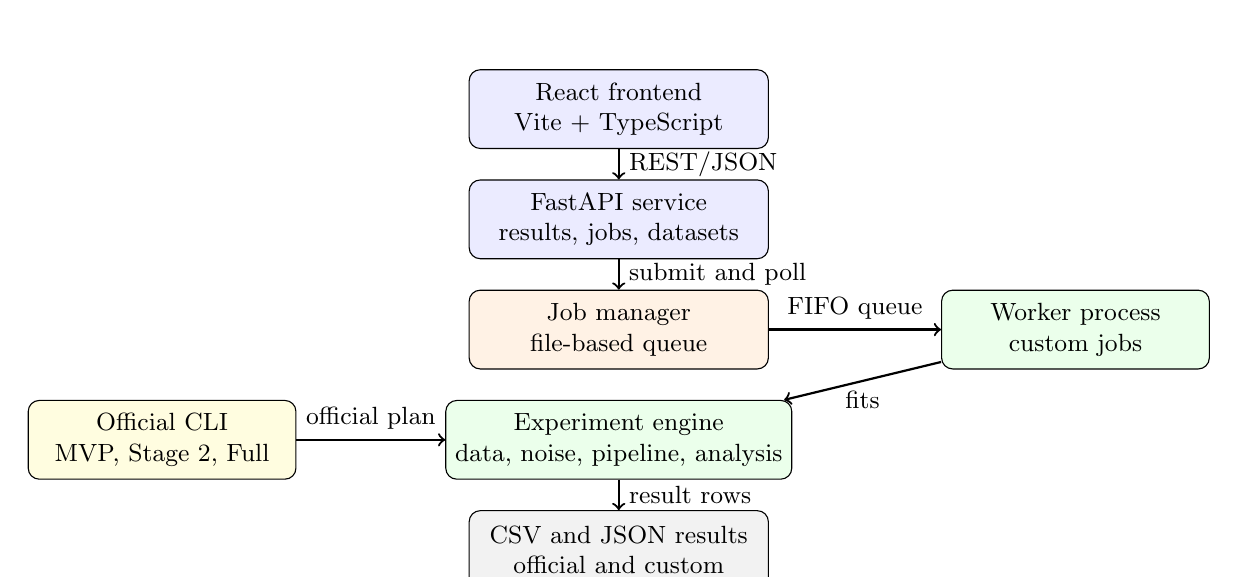
\begin{tikzpicture}[font=\small]
\node[draw, rounded corners, fill=blue!8, minimum width=3.8cm, minimum height=1.0cm, align=center] (ui) at (0,5.6) {React frontend\\Vite + TypeScript};
\node[draw, rounded corners, fill=blue!8, minimum width=3.8cm, minimum height=1.0cm, align=center] (api) at (0,4.2) {FastAPI service\\results, jobs, datasets};
\node[draw, rounded corners, fill=orange!10, minimum width=3.8cm, minimum height=1.0cm, align=center] (jobs) at (0,2.8) {Job manager\\file-based queue};
\node[draw, rounded corners, fill=green!8, minimum width=3.8cm, minimum height=1.0cm, align=center] (engine) at (0,1.4) {Experiment engine\\data, noise, pipeline, analysis};
\node[draw, rounded corners, fill=gray!10, minimum width=3.8cm, minimum height=1.0cm, align=center] (store) at (0,0.0) {CSV and JSON results\\official and custom};
\node[draw, rounded corners, fill=green!8, minimum width=3.4cm, minimum height=1.0cm, align=center] (worker) at (5.8,2.8) {Worker process\\custom jobs};
\node[draw, rounded corners, fill=yellow!12, minimum width=3.4cm, minimum height=1.0cm, align=center] (cli) at (-5.8,1.4) {Official CLI\\MVP, Stage 2, Full};

\draw[->, thick] (ui) -- node[right]{REST/JSON} (api);
\draw[->, thick] (api) -- node[right]{submit and poll} (jobs);
\draw[->, thick] (jobs) -- node[above]{FIFO queue} (worker);
\draw[->, thick] (worker) -- node[below]{fits} (engine);
\draw[->, thick] (cli) -- node[above]{official plan} (engine);
\draw[->, thick] (engine) -- node[right]{result rows} (store);
\end{tikzpicture}}
\caption{High-level system architecture. Official experiments are started from the command line; custom experiments are queued through the API and executed by a separate worker process.}
\label{fig:architecture}
\end{figure}
\section{System Workflow}
For official experiments, the engine loads the datasets and frozen configuration, splits the data, applies training-only corruption, fits each pipeline, and saves metrics and provenance. A separate analysis step produces the benchmark summaries and figures. Custom experiments follow the same approach but are queued through the API.
\section{Use Cases}
A viewer explores results and visualisations. A researcher can select a built-in dataset, use the Covertype preset, or register a CSV and specify its target column before starting a custom run. Official experiments are launched through the command line. The worker processes queued jobs and records their status.
\section{Data Flow}
Dataset and configuration inputs pass through splitting, noise injection, imputation, standardisation and classification. Predictions on the clean test split produce Macro F1 and accuracy. Raw rows feed the baseline, breaking-point, robustness and synergy analyses, which are exposed through the API to the interface.
\section{Data Storage}
The implementation uses files rather than a relational database. Raw results are stored as CSV rows, while manifests, job status and configuration use JSON. Derived CSV files contain summaries, baselines, breaking points, synergy and robustness; hashes and manifests record provenance. JSON writes are atomic and failed fits are recorded.
\section{Module Description}
The data and noise modules prepare inputs; pipeline and runner modules fit models; metrics and analysis modules compute results; storage and figure modules persist and visualise them. The API, worker and frontend connect this engine to the user.

\chapter{Implementation}

\section{Development Environment}

The backend was developed with Python 3.11.9 and the pinned dependencies listed in Chapter~3. The scientific stack is NumPy, pandas, SciPy, and scikit-learn; FastAPI and Uvicorn provide the service layer; Pydantic provides request and response schemas; pytest provides the test suite. The frontend was developed with React, Vite, and TypeScript in strict mode, with Tailwind CSS, shadcn/ui, Lucide icons, Recharts, React Router, and TanStack Query.

The official Full experiment ran on a Windows workstation without a GPU. The run manifest records the Python version, the operating system, the package versions, the Git commit, the frozen configuration hash, the dataset metadata, the model parameters, the seed list, the planned and completed fit counts, and the split hashes for every dataset and seed. This information is sufficient to reconstruct the experimental environment and to verify that a later run used the same methodology.

\section{Module Implementation}

\subsection{Data Module}

The data module loads Breast Cancer and Digits from scikit-learn. It creates a stratified 70/30 split for each $(dataset, seed)$ and returns the clean training and test arrays. It also computes a SHA-256 hash of the training and test indices, which is stored in the manifest. The split is created once and reused for every model, noise type, and combination for that dataset and seed, which is what makes the comparisons paired.

\subsection{Levels and Hashing Module}

The levels module loads the severity table from a JSON configuration file. It validates that the table has the expected keys and that every level vector has six entries (levels 0--5). It exposes the active table and the frozen state. The hashing module computes a canonical JSON representation of the methodology constants, the active level table, the noise order, and the model parameters, and hashes it with SHA-256. The resulting configuration hash is written to every result row and to the manifest. Stage 2, Full, and official resume operations recompute the hash and refuse to run if it does not match the frozen value.

\subsection{Noise Module}

The noise module implements the four injectors. Each injector receives the training features, the training labels, the level value, and a random generator. The generators are created from the seed sequence shown in Chapter~3. Listing~\ref{lst:rng} shows the construction and the identifier mapping.

\begin{lstlisting}[language=Python, caption={Deterministic random generation and noise identifiers.}, label={lst:rng}]
NOISE_IDS = {"label": 1, "gaussian": 2, "outliers": 3, "missing": 4}

def make_rng(seed, noise_name, level):
    return np.random.default_rng(
        np.random.SeedSequence([seed, NOISE_IDS[noise_name], level])
    )
\end{lstlisting}

The label injector flips a fixed number of labels without replacement and always selects a different class. The Gaussian injector scales the standard normal draw by the clean per-column standard deviation and the level factor, and leaves zero-standard-deviation columns unchanged. The outlier injector selects eligible cells and replaces them with a value five standard deviations above or below the column mean. The missing injector sets a Bernoulli-selected subset of cells to NaN.

The compound function applies the injectors in the canonical order:
\begin{center}
\texttt{label} $\rightarrow$ \texttt{gaussian} $\rightarrow$ \texttt{outliers} $\rightarrow$ \texttt{missing}.
\end{center}
The same random generator construction is used for a single noise and for the corresponding component inside a compound, which ensures that the single-noise and compound experiments share the same noise realisation.

\subsection{Pipeline Module}

The pipeline module builds a fresh scikit-learn pipeline for each fit. Listing~\ref{lst:pipeline} shows the structure. The imputer uses mean strategy and keeps empty features so that an entirely missing column does not cause a shape error. The scaler standardises the imputed features. The classifier is one of the four fixed models.

\begin{lstlisting}[language=Python, caption={Preprocessing and classification pipeline.}, label={lst:pipeline}]
from sklearn.impute import SimpleImputer
from sklearn.pipeline import Pipeline
from sklearn.preprocessing import StandardScaler

def build_pipeline(model):
    return Pipeline([
        ("imputer", SimpleImputer(strategy="mean", keep_empty_features=True)),
        ("scaler", StandardScaler()),
        ("model", model),
    ])
\end{lstlisting}

The pipeline is fitted on the training split that is passed to it. At level 0 this is the clean training split; at levels 1--5 it is the corrupted training split. The imputer and scaler therefore learn their statistics from the same data that the classifier sees. No step is fitted on the test set.

\subsection{Metrics Module}

The metrics module computes Macro F1 with \texttt{f1\_score(}\allowbreak\texttt{average="macro",}\allowbreak\texttt{zero\_division=0)} and Accuracy with \texttt{accuracy\_score}. It returns both values together with the fit time. The sample standard deviation in the analysis layer uses \texttt{ddof=1}. Missing predictions or a class with no predicted samples are handled by the zero-division policy rather than by dropping classes.

\subsection{Runner Module}

The runner builds the fit plan for a stage and executes it. A fit plan is a list of fit specifications, each containing the dataset, model, seed, combination, number of noise types, and level. The runner supports resume by reading the completed keys from the raw results file and skipping them. It supports cancellation by checking a flag between fits. Error rows are written with a non-ok status and an error message; they are never removed.

The runner also enforces the frozen configuration guard. Before Stage 2, Full, or an official resume operation, it verifies that the stored configuration hash matches the frozen hash. If the check fails, execution is refused.

\subsection{Analysis Module}

The analysis module reads the raw rows and produces the five derived files. It computes the clean baseline for each dataset and model, the 90\% threshold, the mean and standard deviation by level, the breaking point, the BPI and RS rankings, and the synergy decomposition. The breaking-point computation is shown in Listing~\ref{lst:bp}.

\begin{lstlisting}[language=Python, caption={Breaking-point computation for one dataset, model, and combination.}, label={lst:bp}]
def breaking_point(mean_f1_by_level, baseline_f1, break_ratio=0.90):
    threshold = break_ratio * baseline_f1
    for level in range(1, 6):
        if mean_f1_by_level[level] <= threshold:
            return level
    return None  # not reached
\end{lstlisting}

The function is applied after averaging over seeds. The analysis records whether the breaking point was reached, the F1 at the breaking point, and the number of seeds that were individually below the threshold at that level. This last value distinguishes a consistent failure from a failure driven by one or two seeds.

\subsection{Storage Module}

The storage module defines safe result paths and prevents writes outside the results root. It provides CSV append and read operations and atomic JSON writes. Atomic JSON writes use a temporary file followed by \texttt{os.replace}, which prevents a partially written manifest or job file from being observed. CSV rows are flushed after each fit so that a crash does not lose completed work. The results root can be overridden with the \texttt{RESULTS\_ROOT} environment variable, which allows tests to run against a temporary directory without touching the real results.

\subsection{Figures Module}

The figures module uses matplotlib to generate the official figures from the derived CSVs. It produces F1-versus-level and accuracy-versus-level panels for each single noise, breaking-level heatmaps, a breaking-points table image, and synergy bar charts. The figures use the same model colours and line styles as the frontend so that the report and the application are visually consistent.

\subsection{API Module}

The API module is a FastAPI application with routes for health, configuration, overview statistics, curves, model comparison, breaking points, heatmaps, synergy, experiment listing, experiment detail, experiment creation, cancellation, estimation, and result retrieval. Route handlers validate inputs, call the results reader, and return Pydantic response models. They do not contain machine learning or analysis logic.

\subsection{Worker Module}

The worker is a separate process started with \texttt{python -m app.jobs.worker}. It reads the job queue, executes one custom job at a time, writes progress to the job file, and maintains a heartbeat. Stale running jobs are marked as failed when the worker starts. Cancellation is cooperative and is checked between fits. Partial rows from a cancelled job are preserved and the job ends with the cancelled status.

\subsection{Frontend Module}

The frontend is organised into route-level pages, page-specific feature modules, shared UI components, chart components, hooks, and a typed API client. TanStack Query owns server-state fetching and polling. Polling runs only while a custom job is queued or running. The UI distinguishes official and custom results, shows a provisional banner when the levels are not frozen, and provides loading, empty, and error states for every data view. Colour is never the only carrier of meaning: models also have distinct line styles and markers, and noise types have labels and icons.

\section{User Interface}

The application has six pages. Table~\ref{tab:pages} summarises their purpose.

\begin{table}[H]
\centering
\caption{Application pages.}
\label{tab:pages}
\footnotesize
\begin{tabular}{p{2.2cm}p{3.2cm}p{7.8cm}}
\toprule
\textbf{Page} & \textbf{Route} & \textbf{Purpose} \\
\midrule
Overview & \texttt{/} & Key statistics, robustness ranking, and a short explanation of the experiment \\
Experiment Setup & \texttt{/setup} & Configure a custom experiment, estimate the fit count and runtime, and start it \\
Results Dashboard & \texttt{/results/\allowbreak\{runId\}} & Filterable metrics, level table, and F1-versus-level chart for a run \\
Visualizations & \texttt{/visualizations} & F1 and accuracy curves, model comparison, heatmap, breaking points, and synergy \\
Model Comparison & \texttt{/compare} & Ranking table, robustness highlight, and overlay curves \\
Experiment Details & \texttt{/experiments} and \texttt{/experiments/\allowbreak\{id\}} & Run list, status timeline, configuration, provenance, and manifest download \\
\bottomrule
\end{tabular}
\end{table}

The overview page presents the central result in a compact form: the number of datasets, models, noise types, combinations, total fits, and seeds, followed by the robustness ranking. The results dashboard and the visualizations page provide the detailed evidence. The experiment details page exposes the provenance information that makes the result auditable, including the configuration hash, methodology version, levels version, frozen status, and library versions.

Screenshots of the interface can be added to the report by placing the image files in the \texttt{figures/project\_figures/} directory and including them with the \texttt{figure} environment described in the report README.

\section{Algorithm Implementation}

\subsection{Noise Injection and Fitting}

The complete per-fit algorithm is summarised below.

\begin{enumerate}
  \item Receive the dataset, model, seed, combination, and level.
  \item Load or reuse the stratified split for $(dataset, seed)$.
  \item Copy the clean training features and labels so that the original arrays are not modified.
  \item If the level is 0, fit the pipeline on the clean training split.
  \item Otherwise, for each noise type in the combination, create the generator from $(seed, noise\_id, level)$ and apply the injector to the training data in the canonical order.
  \item Fit the pipeline on the corrupted training data.
  \item Predict the clean test set.
  \item Compute Macro F1, Accuracy, and the fit time.
  \item Record the noise statistics and provenance fields.
  \item Append the row to the raw results file and flush it.
\end{enumerate}

The algorithm is deterministic: the same dataset, model, noise combination, level, and seed produce the same split, the same noise realisation, the same fitted pipeline, and the same metrics. This property was verified by re-running a subset of the Full experiment and comparing the results exactly.

\subsection{Analysis}

The analysis algorithm is:

\begin{enumerate}
  \item Read the raw rows for the run.
  \item Compute the clean baseline and threshold for each dataset and model.
  \item Group the noisy rows by dataset, model, combination, and level, and compute the mean and sample standard deviation over seeds.
  \item For each dataset, model, and combination, scan levels 1--5 and record the first level at or below the threshold.
  \item Compute BPI and RS for the singles and all scopes, and rank the models.
  \item For each compound combination and level, compute the compound drop, the sum of single drops, and the synergy.
  \item Write the derived CSV files and generate the figures.
\end{enumerate}

The analysis is a pure function of the raw rows and the methodology constants. It does not read the test set, does not retrain models, and does not depend on the frontend.

\section{Integration}

The API and worker integrate the engine with the frontend. Table~\ref{tab:api} lists the main endpoints.

\begin{table}[H]
\centering
\caption{Main API endpoints.}
\label{tab:api}
\footnotesize
\begin{tabular}{p{1.4cm}p{5.4cm}p{6.4cm}}
\toprule
\textbf{Method} & \textbf{Endpoint} & \textbf{Purpose} \\
\midrule
GET & \texttt{/api/health} & Server and worker status \\
GET & \texttt{/api/config} & Datasets, models, noise types, levels, frozen state, and available stages \\
GET & \texttt{/api/overview} & Key statistics and robustness ranking \\
POST & \texttt{/api/experiments} & Start a custom run; returns HTTP 202 \\
GET & \texttt{/api/experiments} & List official and custom runs \\
GET & \texttt{/api/experiments/\allowbreak\{id\}} & Status, progress, and manifest summary \\
POST & \texttt{/api/experiments/\allowbreak\{id\}/\allowbreak cancel} & Request cancellation of a custom job \\
GET & \texttt{/api/experiments/\allowbreak\{id\}/\allowbreak results} & Results for a selected run \\
POST & \texttt{/api/experiments/estimate} & Estimate the fit count and runtime of a custom request \\
GET & \texttt{/api/results/curves} & F1 and accuracy versus level \\
GET & \texttt{/api/results/models} & Model comparison and ranking \\
GET & \texttt{/api/\allowbreak results/\allowbreak breaking-points} & Breaking-point table \\
GET & \texttt{/api/results/heatmap} & Model-by-combination breaking-level or retained-F1 grid \\
GET & \texttt{/api/results/synergy} & Synergy analysis for compound combinations \\
\bottomrule
\end{tabular}
\end{table}

For official data, the default stage preference is Full, then Stage 2, then MVP, when no explicit stage is supplied. All endpoints accept optional filters for dataset, model, combination, level, source, stage, and custom run identifier. Errors use a consistent JSON shape with an error code, message, and details. Validation errors return HTTP 422, missing resources return 404, conflicts return 409, and a full queue returns 429.

The integration test for custom experiments starts a small run through the API, monitors it through the worker, and verifies that the official Full results are unchanged. This test is important because it demonstrates the isolation between the official and custom result roots.

\section{Security and Privacy}

The project is designed as a local, single-user research tool. It does not process personal data. The two datasets are public benchmark datasets, and no user accounts, credentials, or personal information are stored. The API is bound to a local development origin, and CORS is restricted to the frontend development origin.

The main security considerations are integrity and isolation rather than confidentiality.

\begin{itemize}
  \item \textbf{Input validation.} Dataset names, model identifiers, noise identifiers, modes, levels, and seed counts are validated against fixed lists and ranges before a job is created.
  \item \textbf{Path safety.} Result paths are constructed from known roots and run identifiers. User-provided names are not used directly as filesystem paths.
  \item \textbf{Official-result protection.} Official runs are started only from the command line. The API has no route that can modify or delete official results. After the final reproducibility check, the official Full directory is locked and its checksums are recorded.
  \item \textbf{Atomic writes.} JSON files are written through a temporary file and an atomic replace, which prevents corrupted manifests or job files.
  \item \textbf{Provenance.} Every result row and manifest records the configuration hash, methodology version, levels version, frozen state, and library versions, which makes tampering or accidental methodology drift visible.
  \item \textbf{No arbitrary code execution.} The API accepts only structured experiment parameters. It does not accept code, file paths, or shell commands from the client.
\end{itemize}

Authentication and authorisation are out of scope for the local version. If the application is deployed on a shared network, the following changes would be required before exposure: authentication, role-based access control, HTTPS, rate limiting, request logging, a restrictive CORS policy, and a review of the worker's filesystem permissions.

\section{Summary}

This chapter described how the methodology is implemented. The engine is modular, deterministic, and testable in isolation. The API exposes read-only results and a controlled custom-experiment workflow. The worker executes custom jobs separately, and the official results are protected by a frozen configuration, atomic writes, and checksums. The frontend presents the results without duplicating any machine learning or analysis logic. The next chapter reports the experimental results obtained from the frozen official Full run.

\chapter{Results and Discussion}

\section{Experimental Setup}

The official experiment uses the two datasets, four classifiers, four noise types, and frozen severity levels described in Chapter~3. The primary metric is Macro F1 and the secondary metric is Accuracy. Every result is evaluated on a clean test set that was never corrupted and never used for fitting.

Table~\ref{tab:runplans} summarises the three official stages and their measured runtimes. The MVP stage is a small Breast Cancer run used for validation and calibration. Stage 2 covers both datasets and all fifteen combinations with seeds 0--2. Full covers both datasets and all fifteen combinations with seeds 0--9.

\begin{table}[H]
\centering
\caption{Official run plans and measured runtimes.}
\label{tab:runplans}
\footnotesize
\begin{tabular}{p{1.1cm}p{1.9cm}p{2.4cm}p{1.1cm}p{1.4cm}p{1.9cm}}
\toprule
\textbf{Stage} & \textbf{Datasets} & \textbf{Combinations} & \textbf{Seeds} & \textbf{Fits} & \textbf{Runtime} \\
\midrule
MVP & Breast Cancer & 4 singles + label + gaussian & 0--2 & 312 & 22.2 s \\
Stage 2 & Both & All 15 & 0--2 & 1,824 & 215.3 s \\
Full & Both & All 15 & 0--9 & 6,080 & 703.8 s \\
\bottomrule
\end{tabular}
\end{table}

All 6,080 Full fits completed with status \texttt{ok} and zero error rows. The mean fit time was 0.1038 seconds and the maximum was 1.1598 seconds. The run used Python 3.11.9 on a Windows workstation without a GPU. The severity table was frozen before Stage 2 with configuration hash \texttt{bc9362\ldots}, methodology version 1.0.0, and levels version 1.0.0. A reproducibility subset of 112 fits was re-run and matched the original results exactly, and SHA-256 checksums were written for the final raw results and manifest.

The split sizes were 398 training and 171 test samples for Breast Cancer, and 1,257 training and 540 test samples for Digits. The same split was reused for every model and noise setting within a dataset and seed, which makes the comparisons paired.

\section{Results}

\subsection{Clean Baselines}

Table~\ref{tab:baselines} reports the clean level-0 baselines and the 90\% thresholds. The baselines are the reference against which every noisy result is compared.

\begin{table}[H]
\centering
\caption{Clean baselines and breaking thresholds (mean over ten seeds).}
\label{tab:baselines}
\small
\begin{tabular}{p{2.3cm}p{3.4cm}p{2.0cm}p{2.4cm}p{2.0cm}}
\toprule
\textbf{Dataset} & \textbf{Model} & \textbf{Baseline F1} & \textbf{Baseline Accuracy} & \textbf{Threshold F1} \\
\midrule
Breast Cancer & Logistic Regression & 0.9700 & 0.9719 & 0.8730 \\
Breast Cancer & SVM (RBF) & 0.9668 & 0.9690 & 0.8701 \\
Breast Cancer & Decision Tree & 0.9272 & 0.9316 & 0.8345 \\
Breast Cancer & Random Forest & 0.9547 & 0.9579 & 0.8592 \\
\midrule
Digits & Logistic Regression & 0.9697 & 0.9696 & 0.8727 \\
Digits & SVM (RBF) & 0.9813 & 0.9813 & 0.8831 \\
Digits & Decision Tree & 0.8420 & 0.8420 & 0.7578 \\
Digits & Random Forest & 0.9747 & 0.9748 & 0.8773 \\
\bottomrule
\end{tabular}
\end{table}

On Breast Cancer, Logistic Regression has the highest clean Macro F1 (0.9700), followed closely by SVM (0.9668) and Random Forest (0.9547). The Decision Tree is the weakest at 0.9272. On Digits, SVM is strongest (0.9813), followed by Random Forest (0.9747) and Logistic Regression (0.9697); the Decision Tree is again the weakest at 0.8420. The Decision Tree's lower baseline means that its threshold is also lower, so its early breaking points are not merely an artefact of a stricter absolute threshold.

\subsection{Breaking Points for Single Noise}

Table~\ref{tab:singlebp} reports the breaking level for each dataset, model, and single noise. ``NR'' means that the model did not reach the threshold by level 5.

\begin{table}[H]
\centering
\caption{Breaking levels for the four single-noise combinations (NR = not reached).}
\label{tab:singlebp}
\small
\begin{tabular}{llcccc}
\toprule
\textbf{Dataset} & \textbf{Model} & \textbf{Label} & \textbf{Gaussian} & \textbf{Outliers} & \textbf{Missing} \\
\midrule
Breast Cancer & Logistic Regression & 5 & NR & NR & NR \\
Breast Cancer & SVM (RBF) & 5 & NR & NR & NR \\
Breast Cancer & Decision Tree & 2 & 5 & NR & NR \\
Breast Cancer & Random Forest & 5 & 5 & NR & NR \\
\midrule
Digits & Logistic Regression & 4 & NR & NR & NR \\
Digits & SVM (RBF) & NR & NR & 5 & NR \\
Digits & Decision Tree & 2 & 3 & NR & 3 \\
Digits & Random Forest & NR & 5 & NR & NR \\
\bottomrule
\end{tabular}
\end{table}

The table reveals a clear ordering. Label noise is the most damaging single corruption. Averaged over the eight dataset--model pairs and treating ``not reached'' as level 6, the mean breaking level is 4.375 for label noise, 5.250 for Gaussian noise, 5.625 for missing values, and 5.875 for outliers. The corresponding mean absolute Macro F1 drop at level 5 is 0.1808 for label noise, 0.1251 for Gaussian noise, 0.0531 for missing values, and 0.0430 for outliers.

Label noise breaks every model on Breast Cancer and three of four models on Digits. Gaussian noise is the second most damaging corruption, and it breaks the Decision Tree and Random Forest on both datasets. Outliers and missing values rarely break a model in isolation, although missing values break the Decision Tree on Digits at level 3. SVM is unusually robust to label noise on Digits, where it does not reach the threshold by level 5, but it is the only model that breaks under outliers alone on Digits, at level 5.

\subsection{Compound-Noise Effects}

Compound noise is consistently more harmful than single noise. Table~\ref{tab:compoundbp} reports the mean breaking level by number of noise types, again treating ``not reached'' as level 6.

\begin{table}[H]
\centering
\caption{Mean breaking level by noise-set size (NR = 6).}
\label{tab:compoundbp}
\small
\begin{tabular}{lcccc}
\toprule
\textbf{Dataset} & \textbf{Singles} & \textbf{Pairs} & \textbf{Triples} & \textbf{Four-way} \\
\midrule
Breast Cancer & 5.438 & 5.208 & 4.875 & 4.750 \\
Digits & 5.125 & 4.250 & 3.562 & 2.750 \\
Combined & 5.281 & 4.729 & 4.219 & 3.750 \\
\bottomrule
\end{tabular}
\end{table}

The monotonic decrease is the central empirical result of the project. On Breast Cancer, the mean breaking level falls from 5.438 for single noise to 5.208 for pairs, 4.875 for triples, and 4.750 for the four-way combination. On Digits the decline is much steeper: 5.125, 4.250, 3.562, and 2.750. The four-way combination is therefore the most damaging setting in the entire experiment, and the gap between the single-noise and four-way means is 1.531 levels when the two datasets are combined.

Table~\ref{tab:keycombos} reports the mean breaking level for selected combinations on each dataset. It shows that combinations containing label noise dominate the early-failure region, and that the four-way combination is the earliest-breaking combination on Digits.

\begin{table}[H]
\centering
\caption{Mean breaking level for selected combinations (NR = 6).}
\label{tab:keycombos}
\footnotesize
\begin{tabular}{lccc}
\toprule
\textbf{Combination} & \textbf{Breast Cancer} & \textbf{Digits} & \textbf{Combined} \\
\midrule
Label & 4.250 & 4.500 & 4.375 \\
Gaussian & 5.500 & 5.000 & 5.250 \\
Missing & 6.000 & 5.250 & 5.625 \\
Outliers & 6.000 & 5.750 & 5.875 \\
Label + Gaussian & 4.750 & 4.250 & 4.500 \\
Label + Gaussian + Missing & 4.500 & 3.500 & 4.000 \\
Label + Gaussian + Outliers & 4.750 & 3.500 & 4.125 \\
Label + Outliers + Missing & 4.500 & 3.750 & 4.125 \\
Gaussian + Outliers + Missing & 5.750 & 3.500 & 4.625 \\
Label + Gaussian + Outliers + Missing & 4.750 & 2.750 & 3.750 \\
\bottomrule
\end{tabular}
\end{table}

Across all 120 dataset--model--combination cells, 83 breaking points were reached and 37 were not. Of the reached breaking points, 8 occurred at level 2, 15 at level 3, 22 at level 4, and 38 at level 5. The distribution differs sharply between datasets. On Breast Cancer, 28 of the 36 reached breaking points occurred at level 5, which indicates a late and gradual failure. On Digits, only 10 of the 47 reached breaking points occurred at level 5, while 19 occurred at level 4, 12 at level 3, and 6 at level 2, which indicates earlier and more abrupt failure.

\subsection{Robustness Ranking}

Table~\ref{tab:robustness} reports the BPI, RS, and rank for the all-combinations and single-noise scopes. Higher BPI means that a model survives to a higher severity; higher RS means that it retains more of its baseline performance across levels.

\begin{table}[H]
\centering
\caption{Robustness ranking by BPI and RS.}
\label{tab:robustness}
\resizebox{\textwidth}{!}{%
\begin{tabular}{llcccccc}
\toprule
\textbf{Dataset} & \textbf{Model} & \textbf{BPI (all)} & \textbf{RS (all)} & \textbf{Rank} & \textbf{BPI (singles)} & \textbf{RS (singles)} & \textbf{Rank} \\
\midrule
Breast Cancer & Logistic Regression & 5.467 & 0.960 & 1 & 5.750 & 0.972 & 2 \\
Breast Cancer & SVM (RBF) & 5.467 & 0.958 & 2 & 5.750 & 0.976 & 1 \\
Breast Cancer & Random Forest & 5.400 & 0.957 & 3 & 5.500 & 0.968 & 3 \\
Breast Cancer & Decision Tree & 4.267 & 0.895 & 4 & 4.750 & 0.931 & 4 \\
\midrule
Digits & Random Forest & 4.800 & 0.922 & 1 & 5.750 & 0.975 & 1 \\
Digits & Logistic Regression & 4.667 & 0.925 & 2 & 5.500 & 0.953 & 3 \\
Digits & SVM (RBF) & 4.533 & 0.922 & 3 & 5.750 & 0.966 & 2 \\
Digits & Decision Tree & 2.800 & 0.747 & 4 & 3.500 & 0.862 & 4 \\
\bottomrule
\end{tabular}}
\end{table}

No single model dominates on both datasets. On Breast Cancer, Logistic Regression and SVM have the same all-combination BPI (5.467), and Logistic Regression is ranked first by the RS tie-break. On Digits, Random Forest is ranked first with BPI 4.800 and RS 0.922. The Decision Tree is last on both datasets, with a BPI of 4.267 on Breast Cancer and 2.800 on Digits. Its RS is also the lowest: 0.895 on Breast Cancer and 0.747 on Digits.

Averaged across the two datasets, Random Forest has the highest mean BPI (5.100), followed by Logistic Regression (5.067), SVM (5.000), and Decision Tree (3.533). Logistic Regression has the highest mean RS (0.9423), followed by Random Forest (0.9397), SVM (0.9396), and Decision Tree (0.8207). The two aggregate measures therefore agree on the weakest model and disagree slightly on the strongest, which is why both are reported.

\subsection{Synergy Analysis}

The synergy analysis compares the compound drop with the sum of the corresponding single-noise drops. A positive value means that the compound is worse than additive; a negative value means that it is less than additive. The analysis covers 440 compound cells: 11 compound combinations, 4 models, 2 datasets, and 5 levels.

Of the 440 cells, 124 (28.2\%) have positive synergy and 316 (71.8\%) have negative synergy. The mean synergy is negative on both datasets: $-0.0308$ on Breast Cancer and $-0.0105$ on Digits. At level 5, the mean is $-0.0711$ on Breast Cancer and $-0.0024$ on Digits. The general pattern is therefore sub-additive: the damage caused by compound noise is usually smaller than the sum of the damage caused by the same noises individually.

The exceptions are important. The largest positive synergy is 0.2958, for Random Forest on Digits with the four-way combination at level 5. The next largest are 0.1601 for SVM on Digits with label + Gaussian + outliers at level 5, and 0.0672 for SVM on Breast Cancer with label + Gaussian + outliers at level 5. These are cases in which the interaction between corruption types produces more damage than an additive model would predict. The floor-effect flag is set in two cases, both for the Decision Tree on Digits at level 5, where the sum of single-noise drops exceeds the baseline.

The practical implication is that compound noise is more damaging in absolute terms, but not necessarily more than additive. A simple additive projection can overestimate the total drop in most cells, while underestimating it in a small number of high-severity multiclass cells. Both the absolute effect and the interaction effect should therefore be reported.

\subsection{Figures}

Figures~\ref{fig:bc-f1} and~\ref{fig:digits-f1} show Macro F1 versus severity for each single noise. Each panel contains the four models, the mean over ten seeds, a shaded one-standard-deviation band, the 90\% threshold, and a red cross at the breaking point.

\begin{figure}[H]
\centering
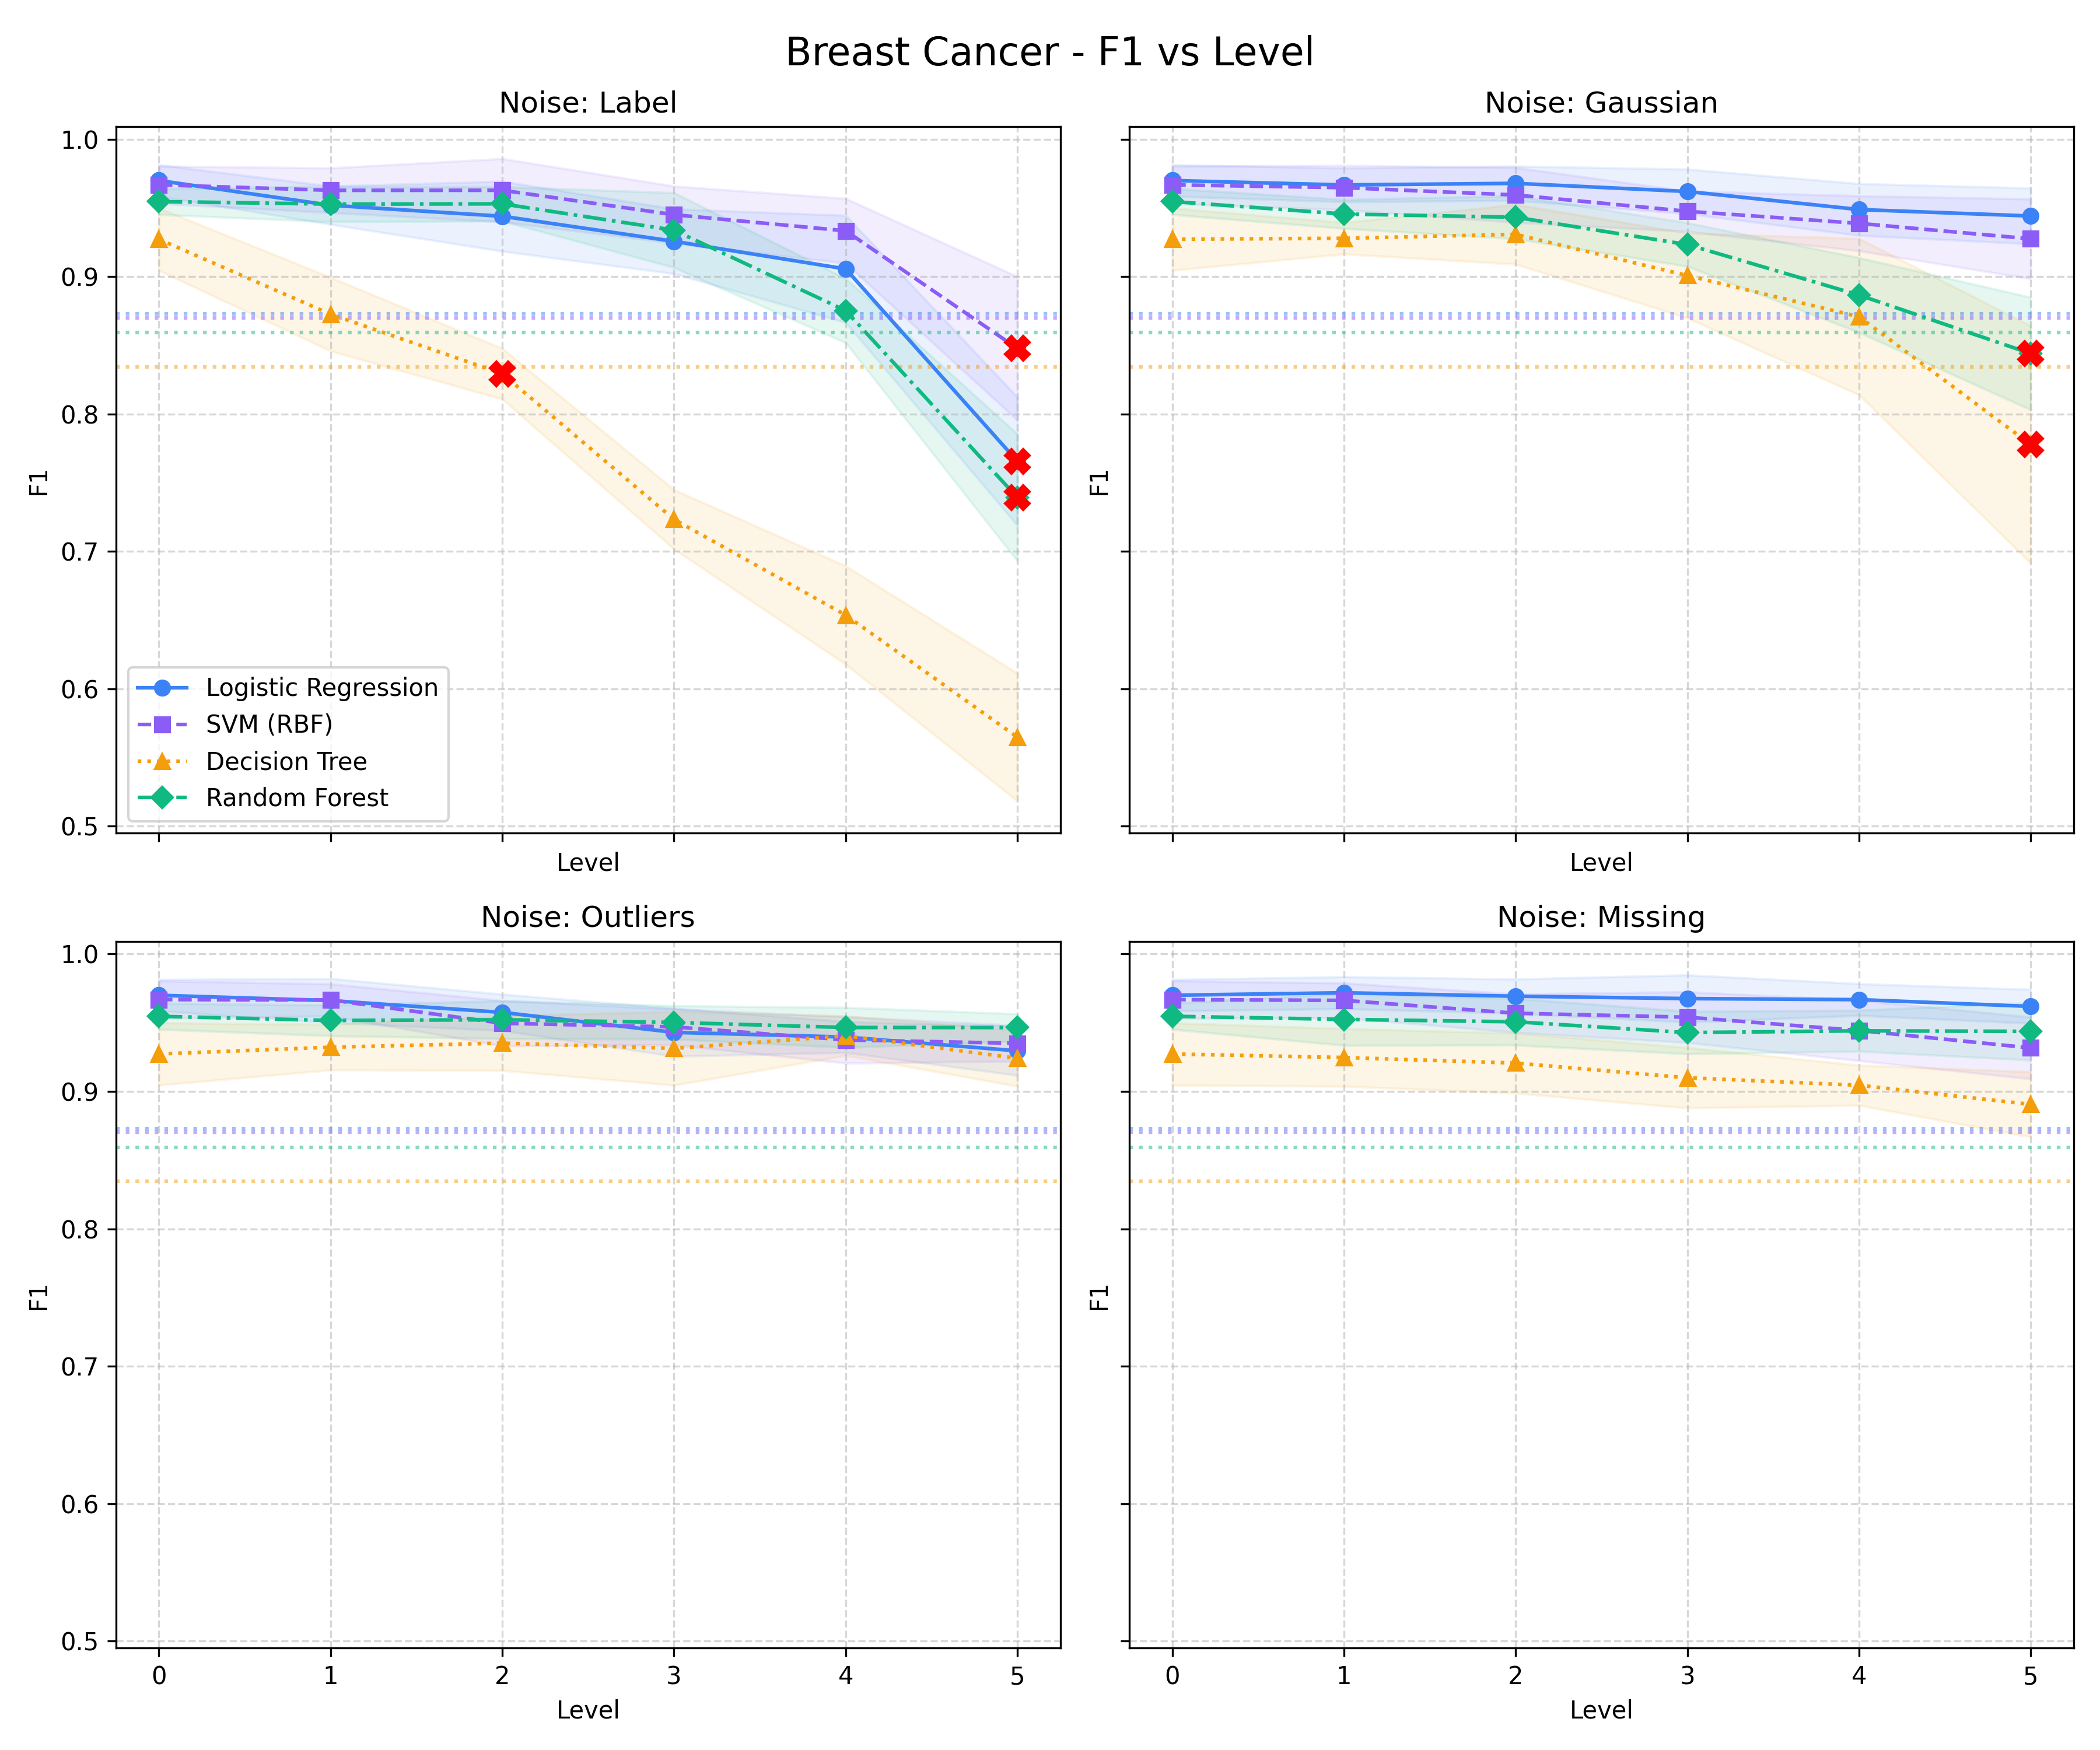
\includegraphics[width=0.95\textwidth]{figures/project_figures/bc-f1-vs-level.png}
\caption{Breast Cancer: Macro F1 versus severity level for the four single-noise combinations. The dotted lines are the 90\% thresholds and the red crosses mark breaking points.}
\label{fig:bc-f1}
\end{figure}

\begin{figure}[H]
\centering
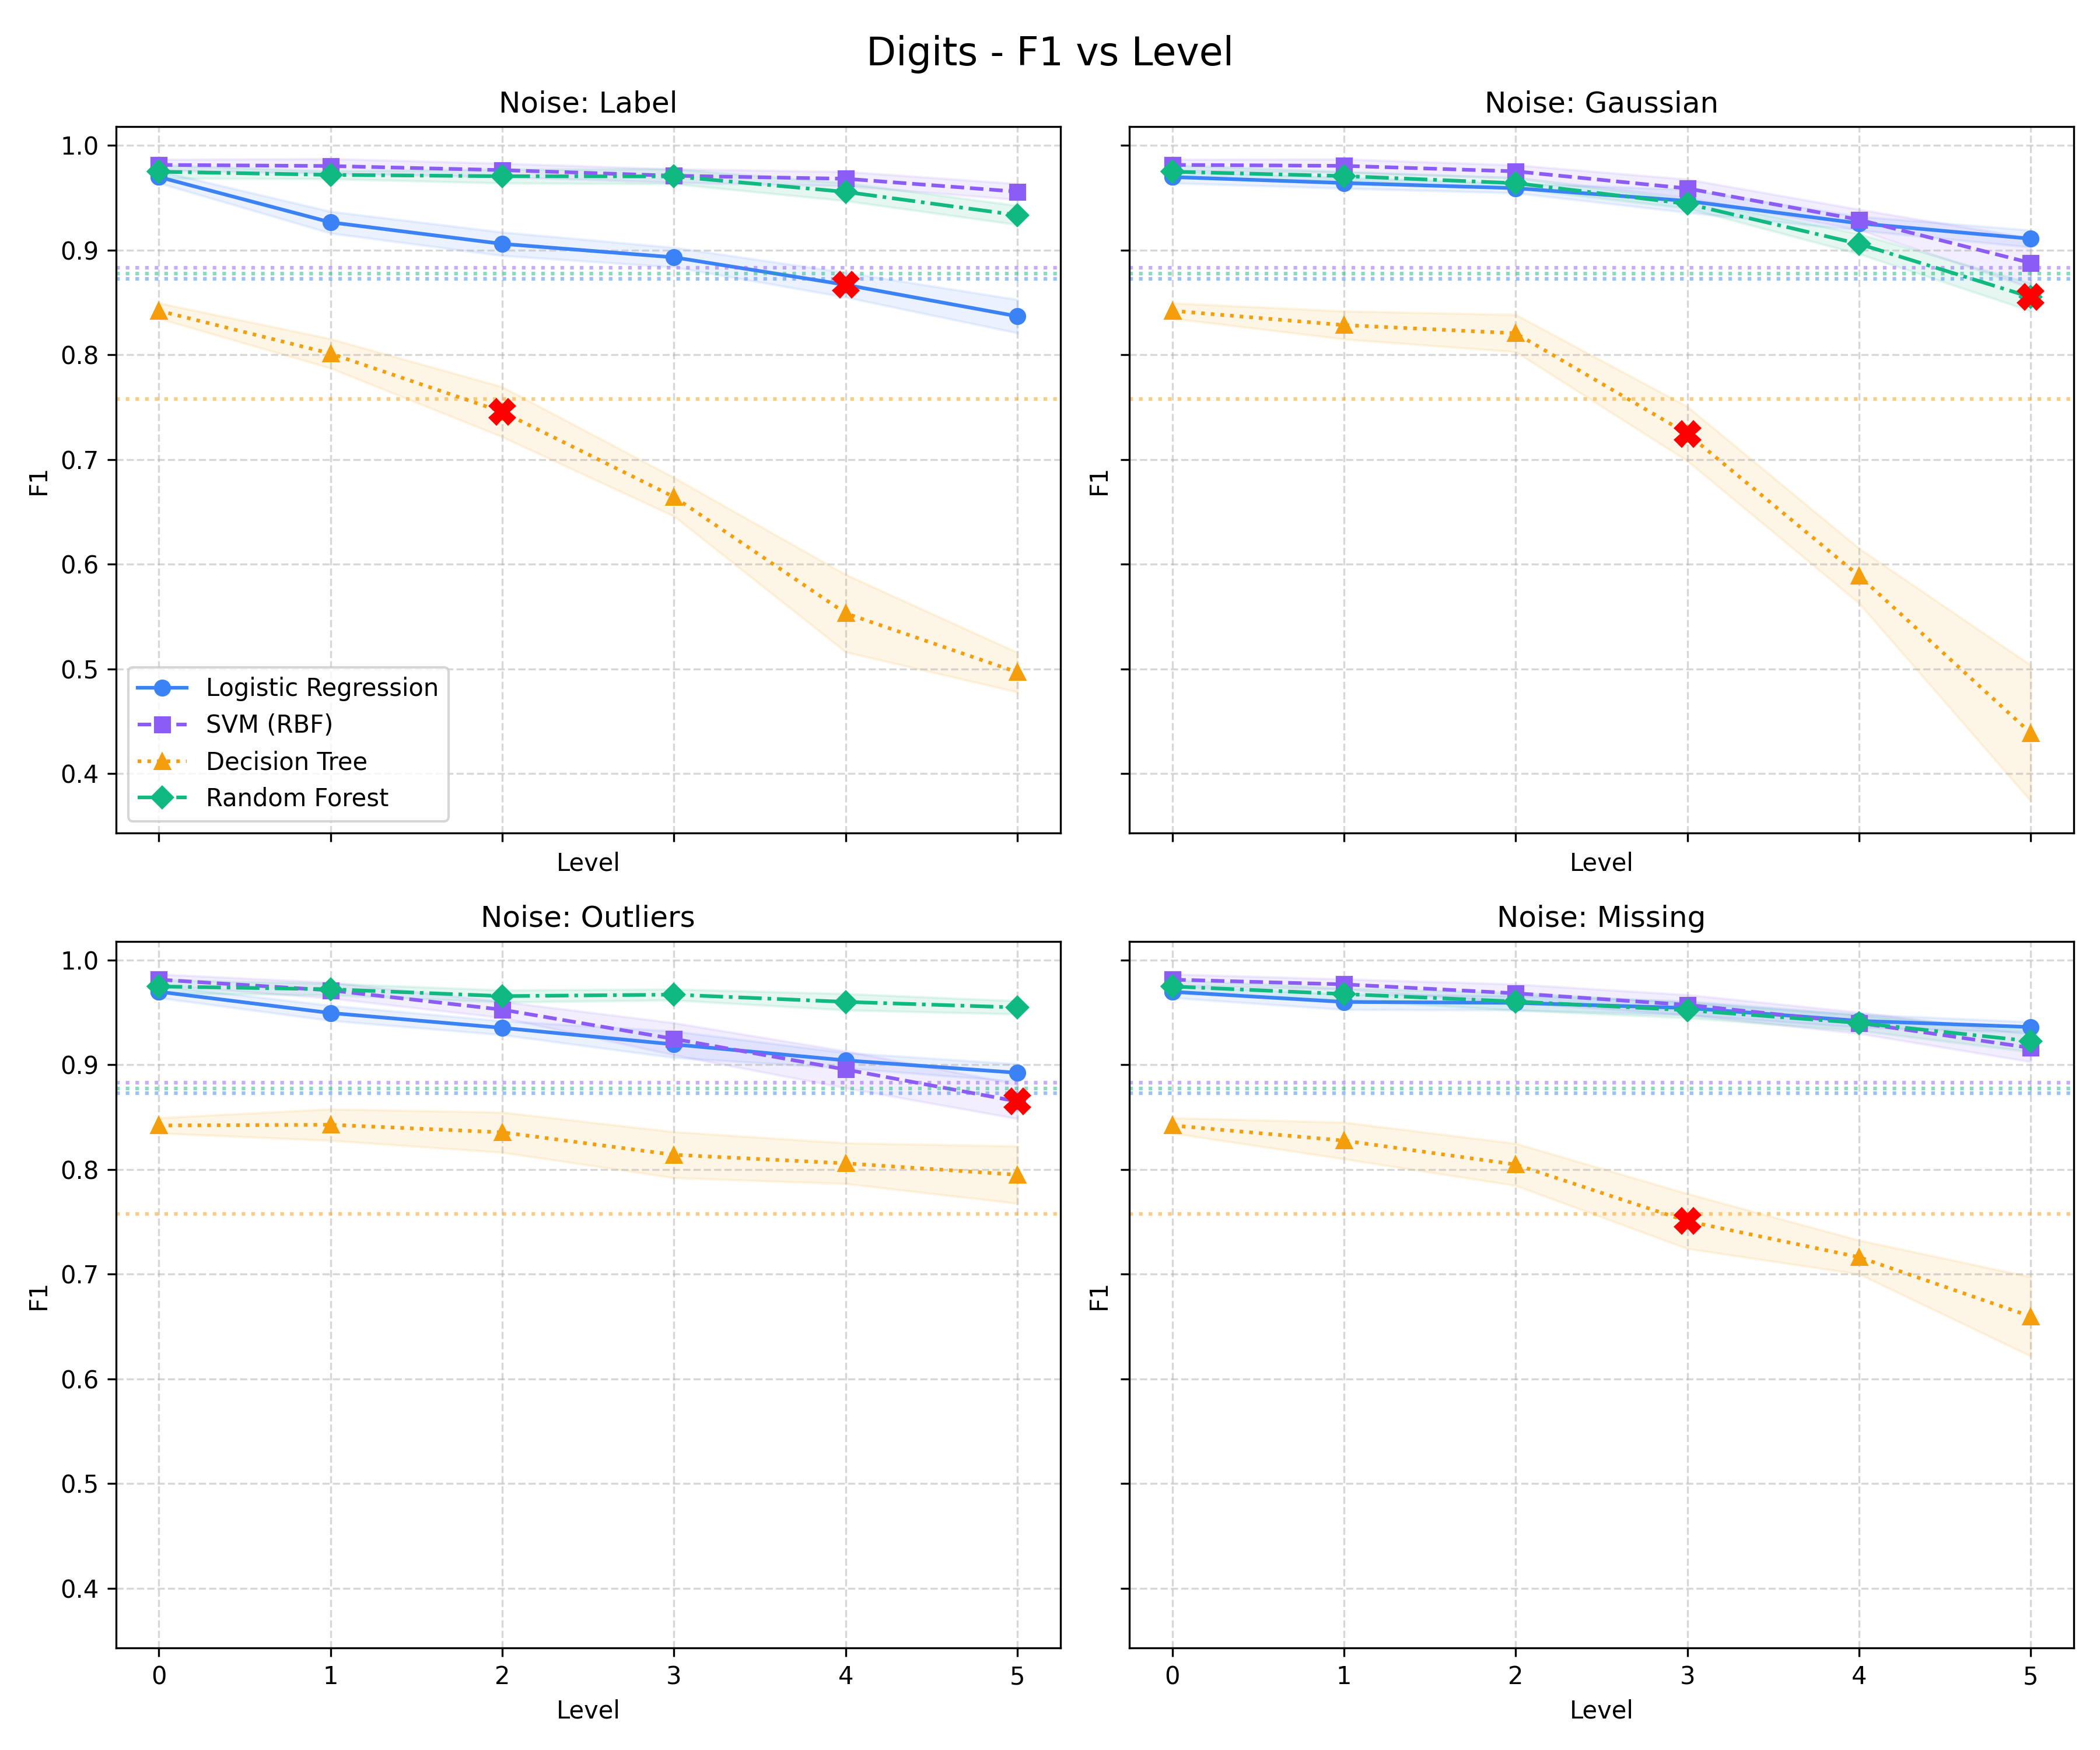
\includegraphics[width=0.95\textwidth]{figures/project_figures/digits-f1-vs-level.png}
\caption{Digits: Macro F1 versus severity level for the four single-noise combinations. The dotted lines are the 90\% thresholds and the red crosses mark breaking points.}
\label{fig:digits-f1}
\end{figure}

Figures~\ref{fig:bc-heat} and~\ref{fig:digits-heat} show the breaking level for all fifteen combinations and four models. Lighter cells indicate earlier failure, darker cells indicate later failure, and the value 6 means that the threshold was not reached.

\begin{figure}[H]
\centering
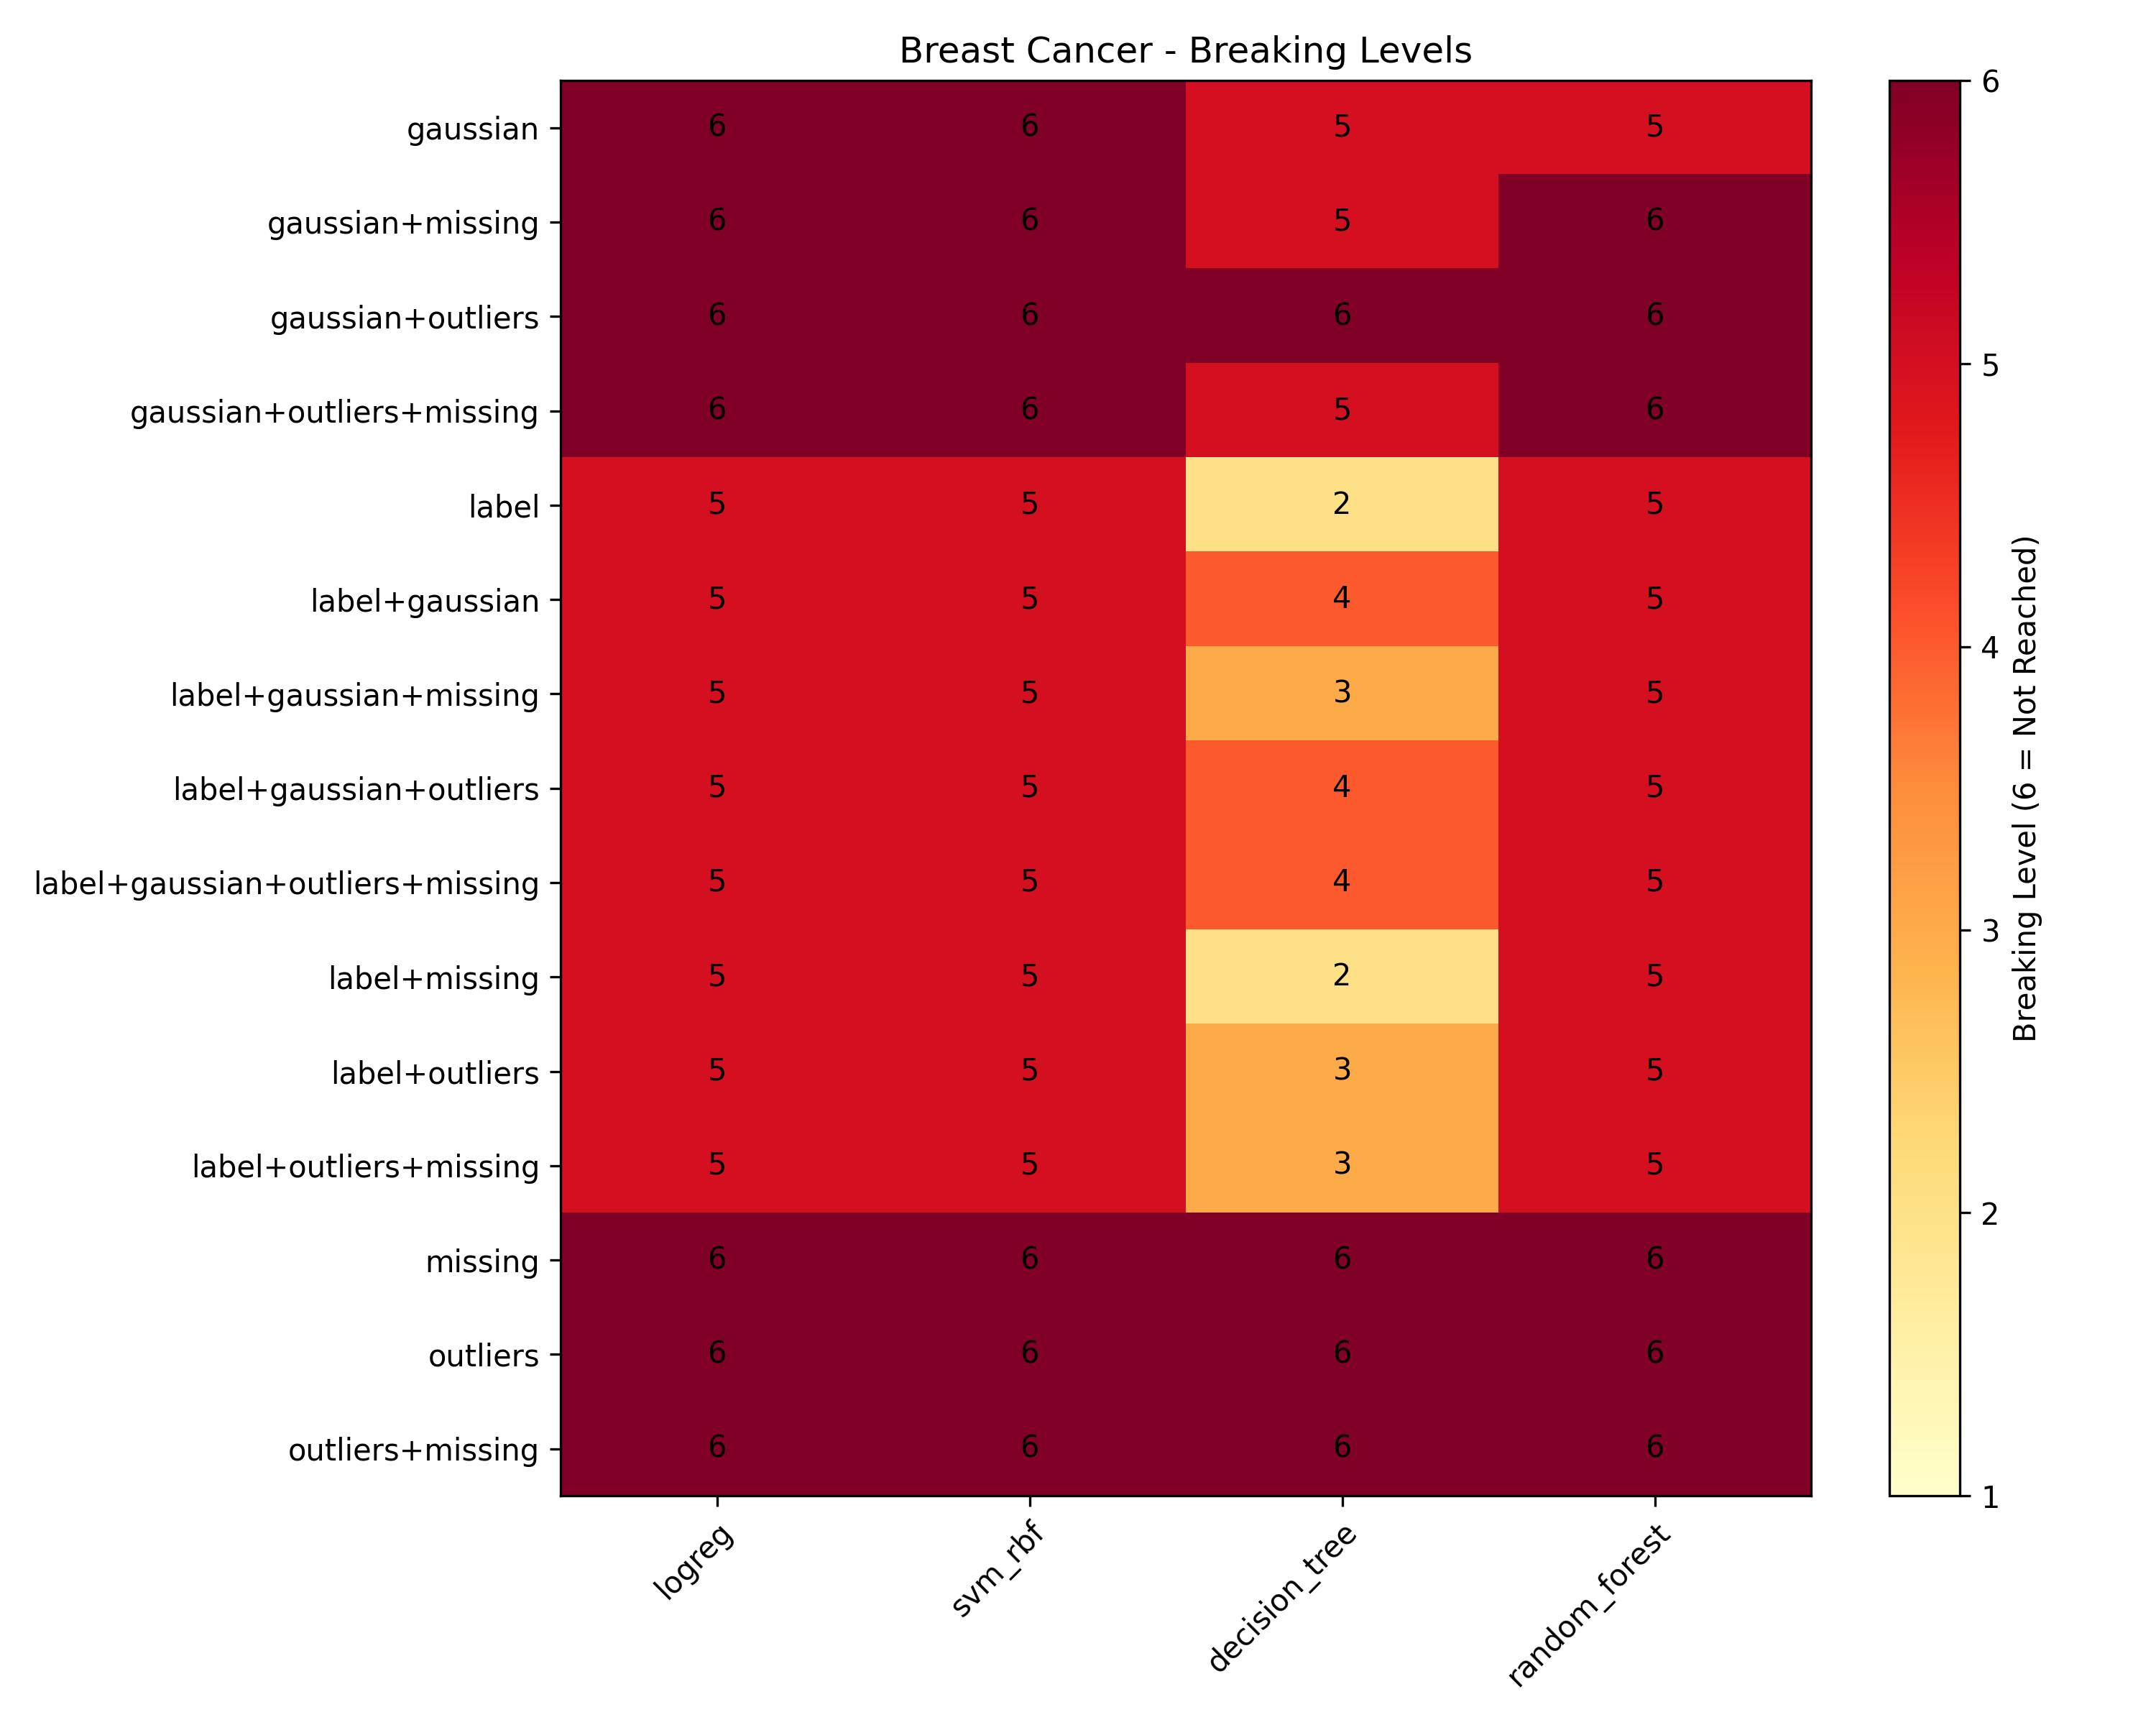
\includegraphics[width=0.82\textwidth]{figures/project_figures/bc-heatmap.png}
\caption{Breast Cancer: breaking level for every combination and model. Lighter cells fail earlier; 6 means not reached.}
\label{fig:bc-heat}
\end{figure}

\begin{figure}[H]
\centering
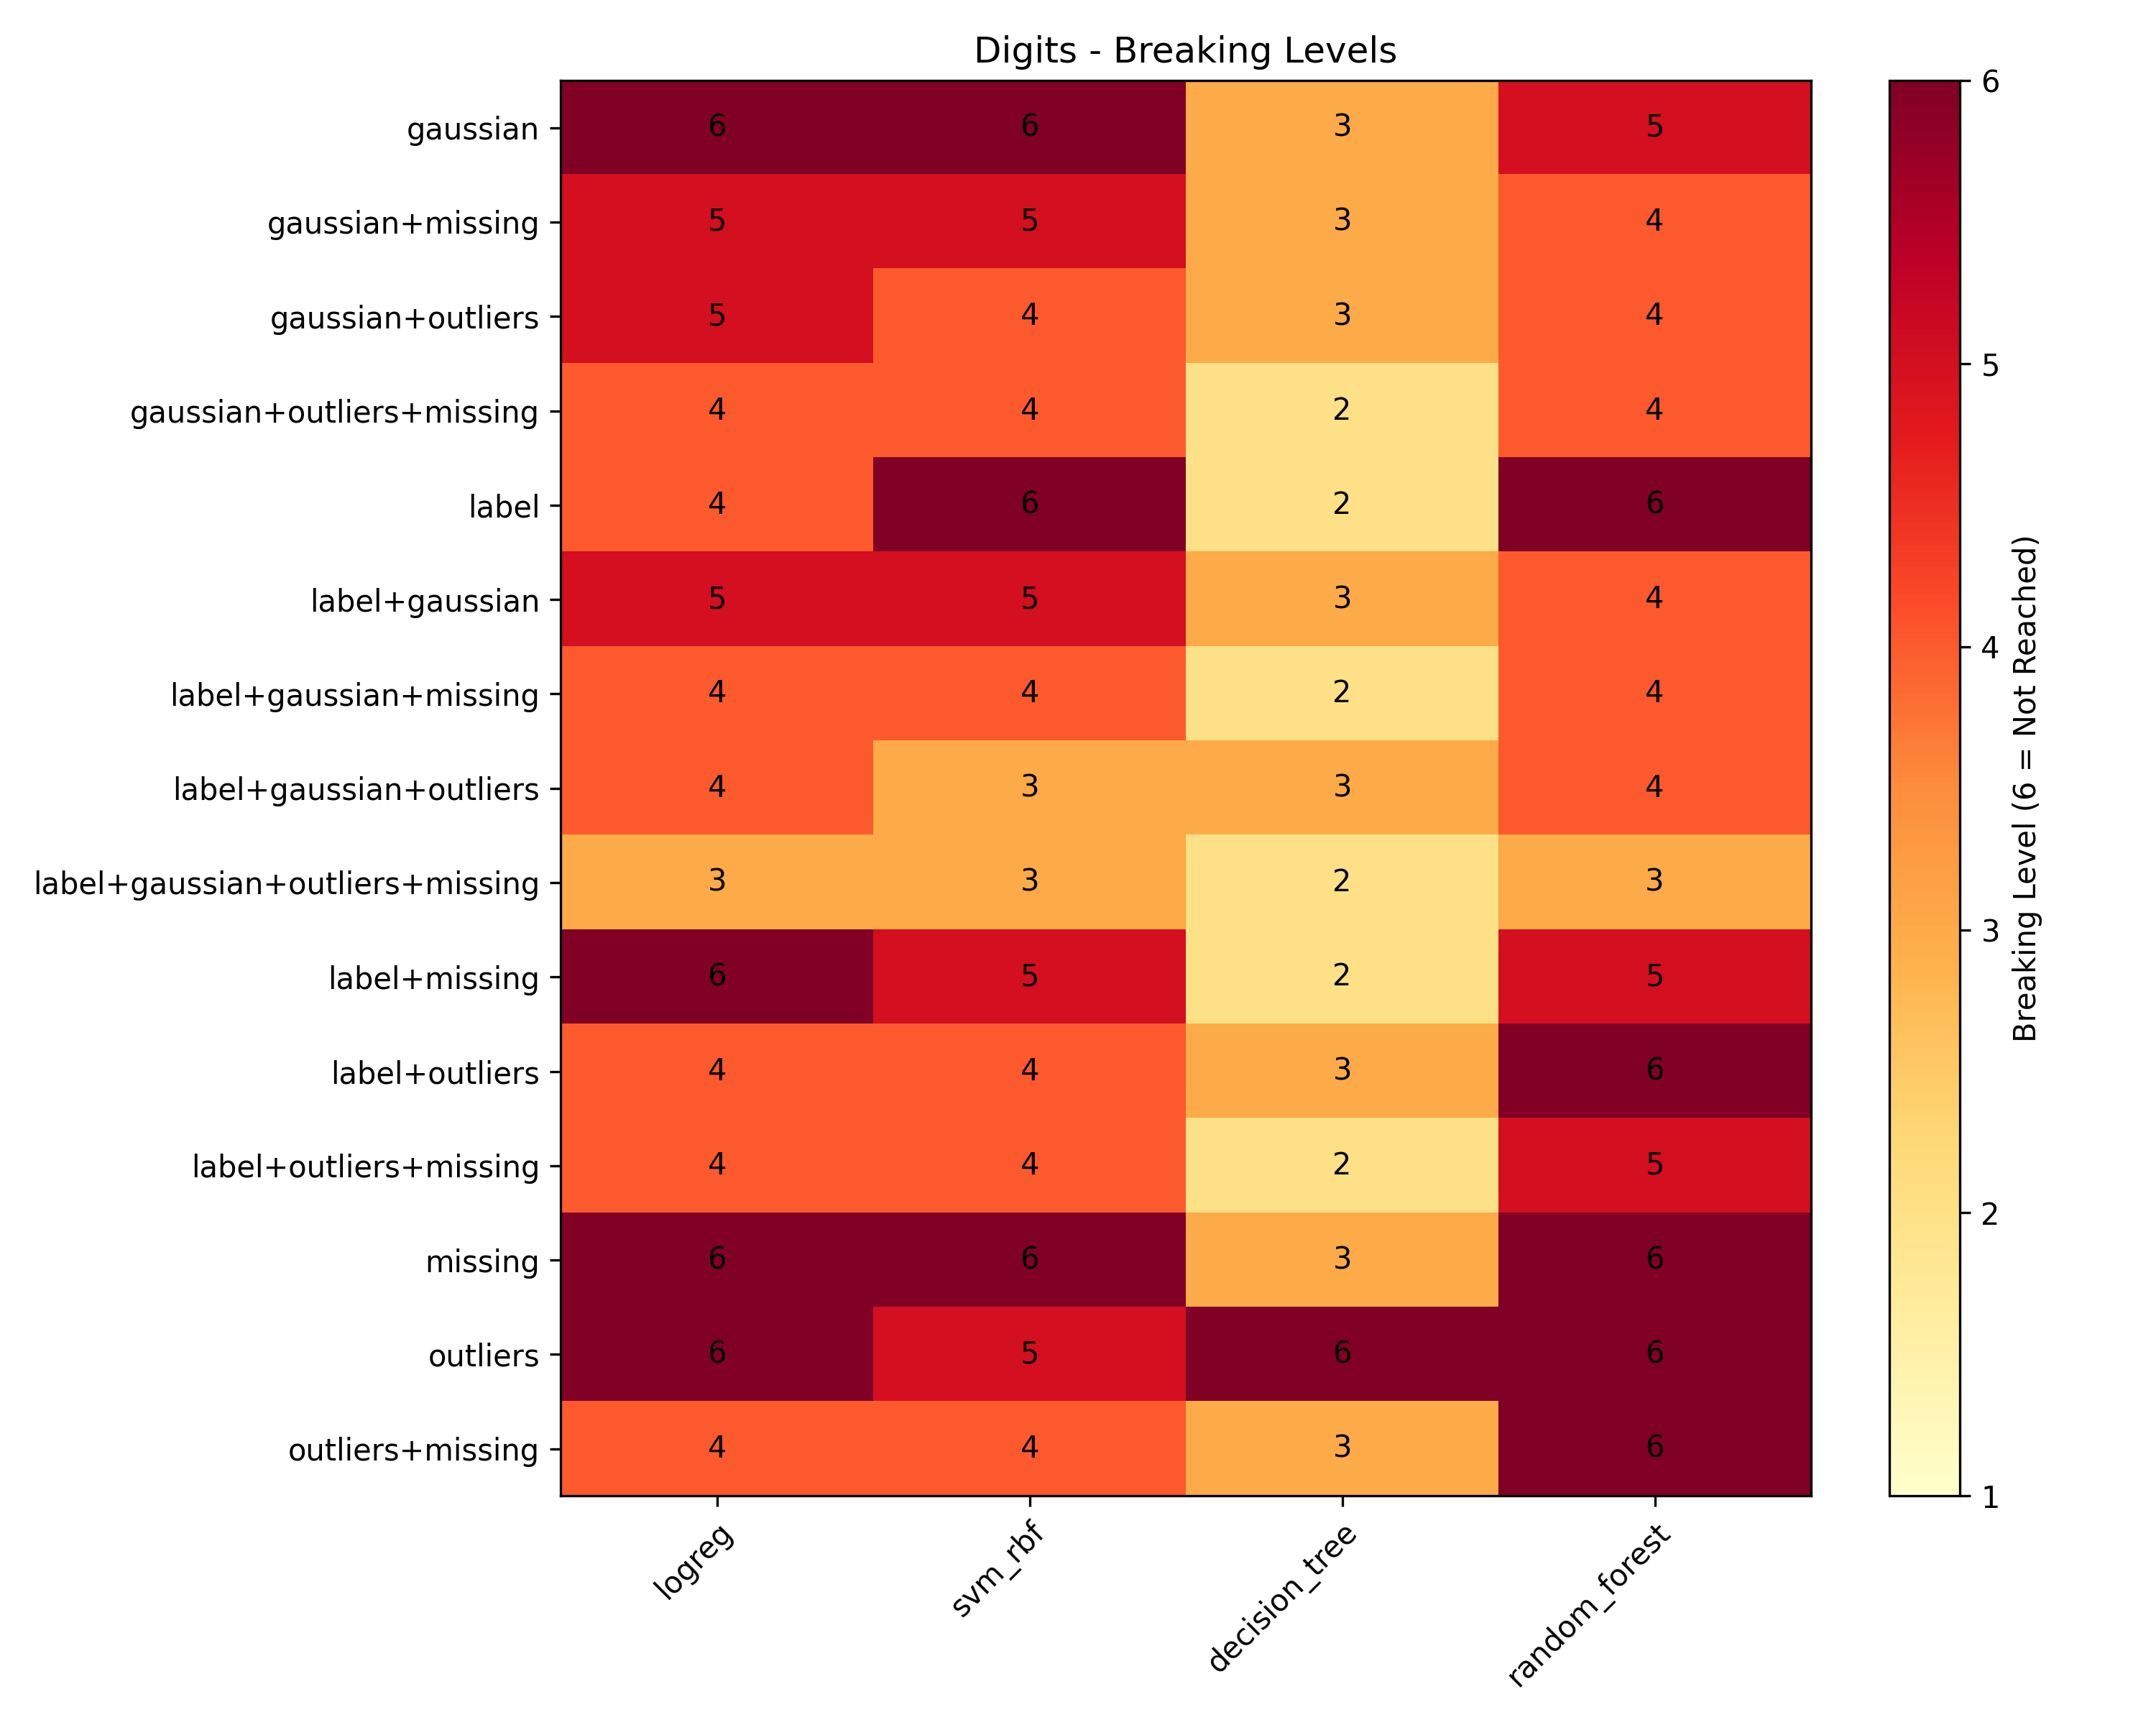
\includegraphics[width=0.82\textwidth]{figures/project_figures/digits-heatmap.png}
\caption{Digits: breaking level for every combination and model. The much lighter cells show earlier failure than on Breast Cancer.}
\label{fig:digits-heat}
\end{figure}

Figures~\ref{fig:bc-syn} and~\ref{fig:digits-syn} show the level-5 synergy for every compound combination and model. Positive bars indicate super-additive damage.

\begin{figure}[H]
\centering
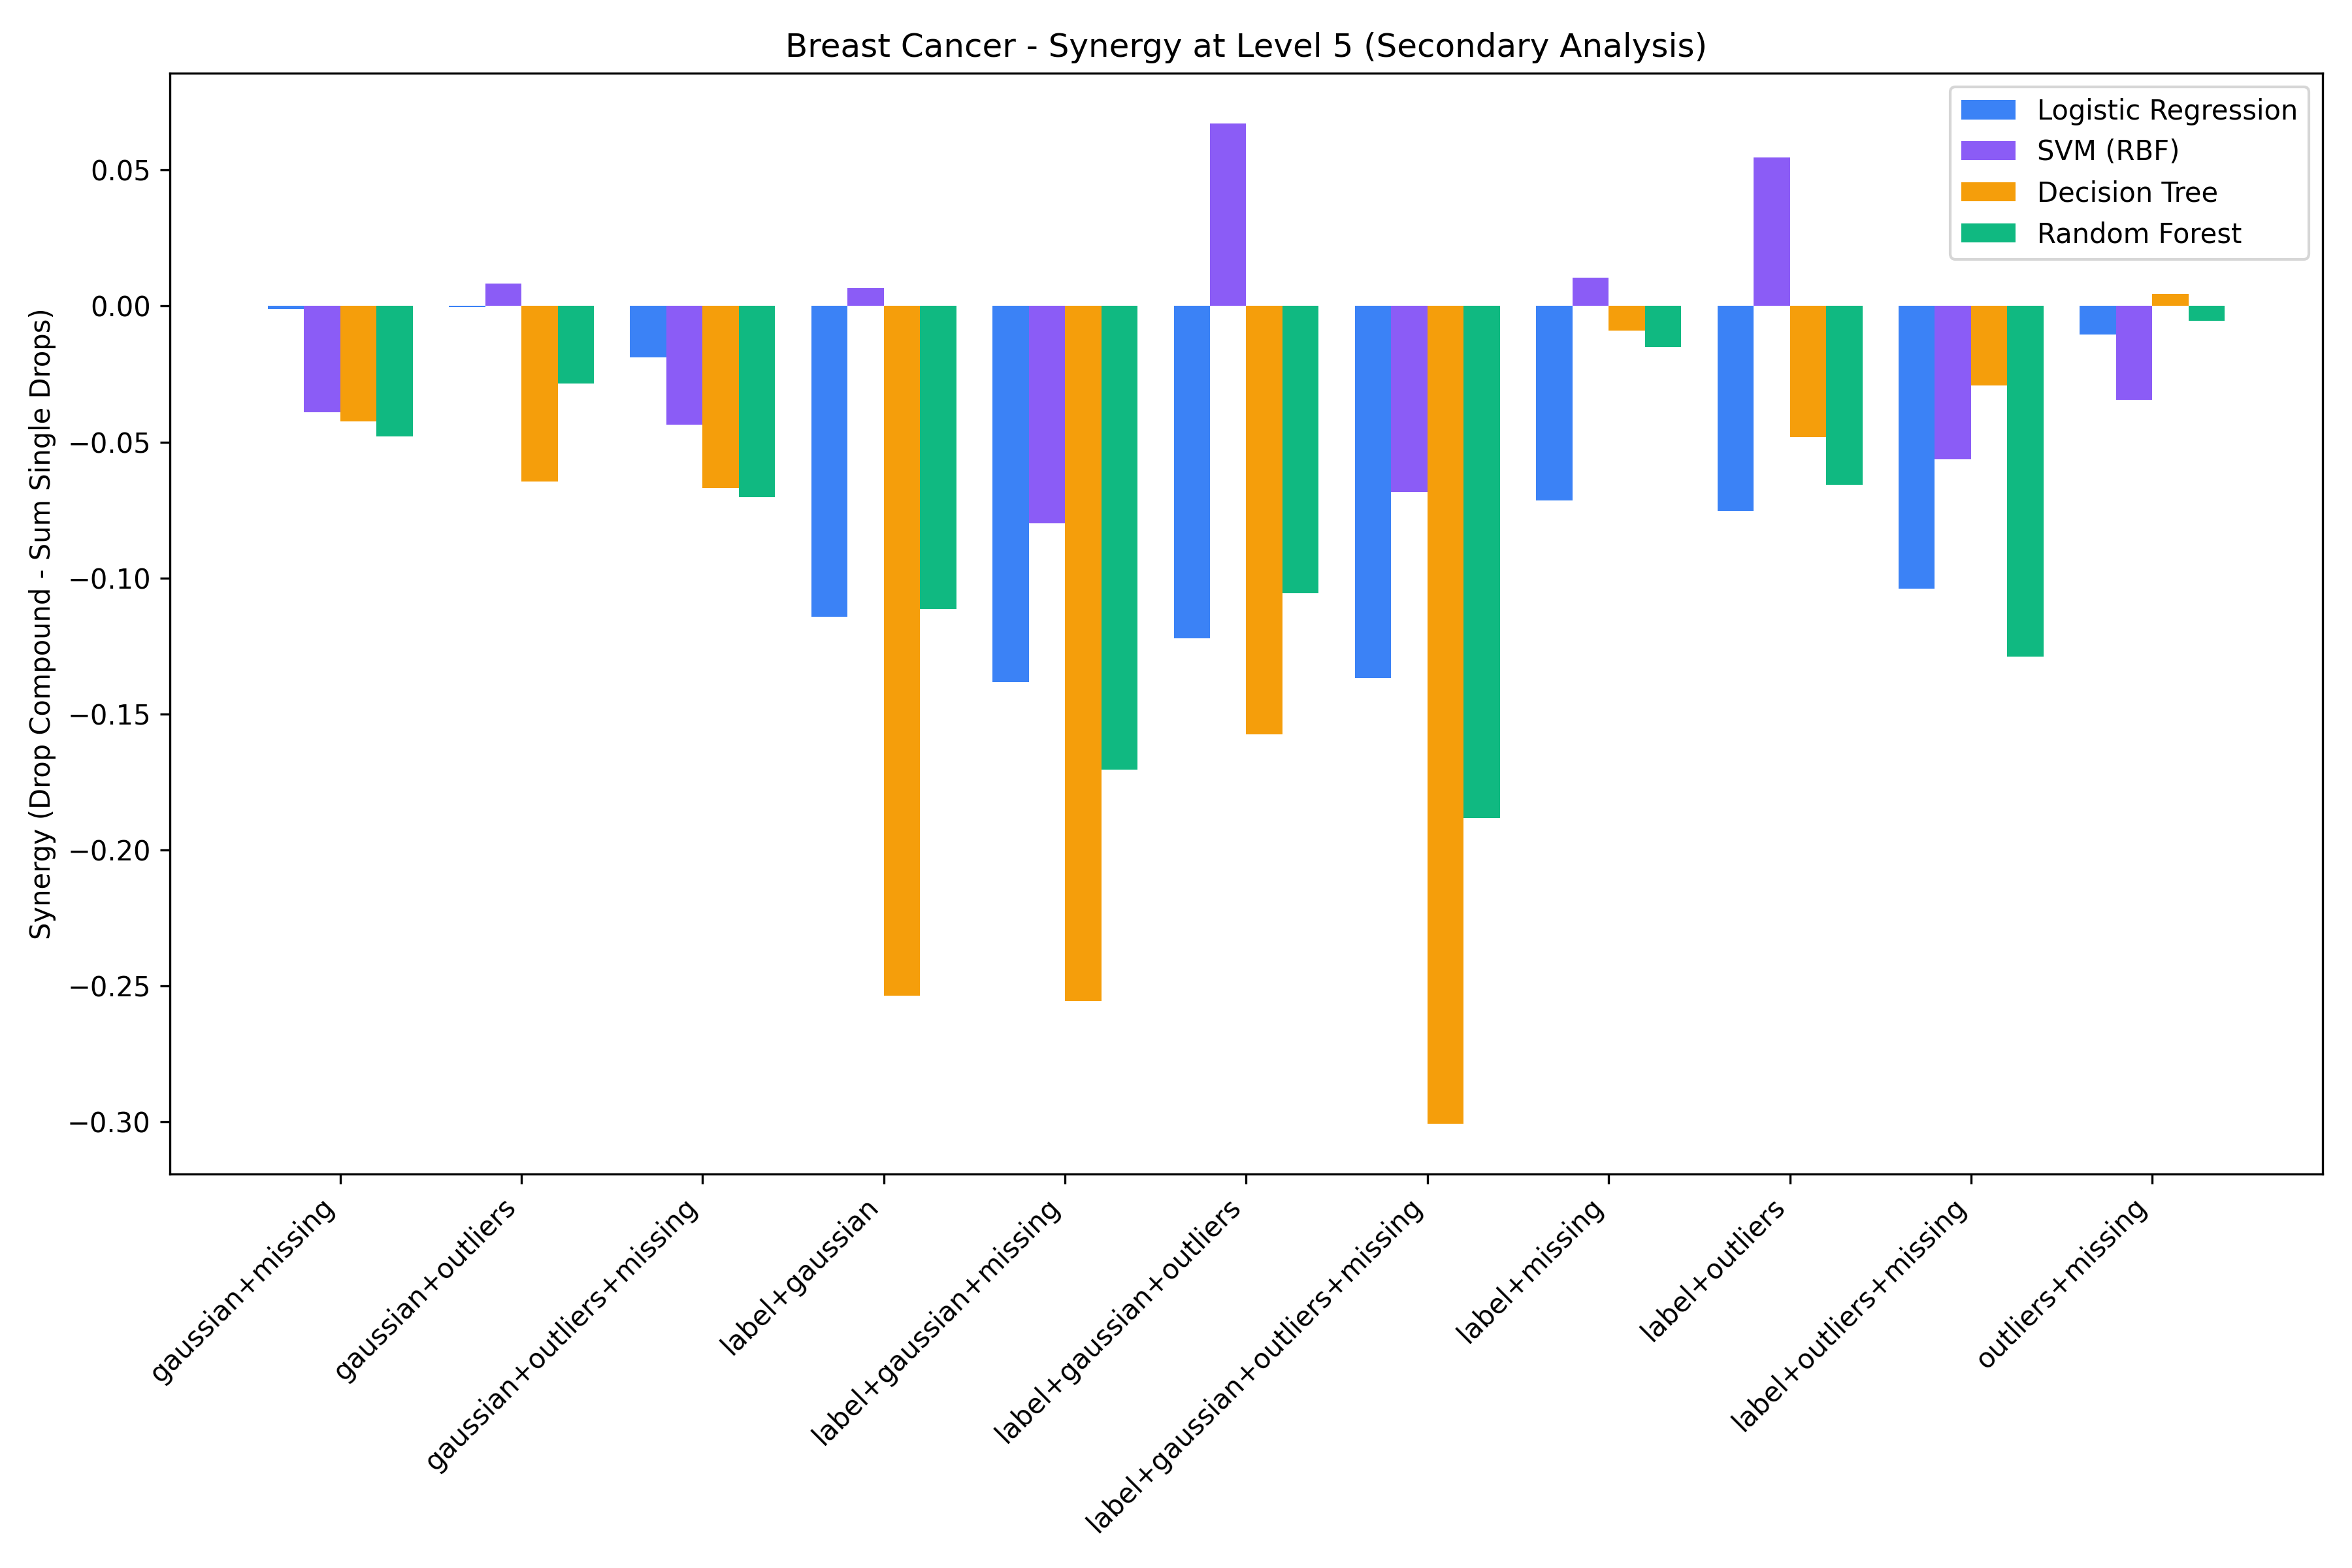
\includegraphics[width=0.95\textwidth]{figures/project_figures/bc-synergy.png}
\caption{Breast Cancer: synergy at level 5. Positive values mean that the compound drop exceeds the sum of single-noise drops.}
\label{fig:bc-syn}
\end{figure}

\begin{figure}[H]
\centering
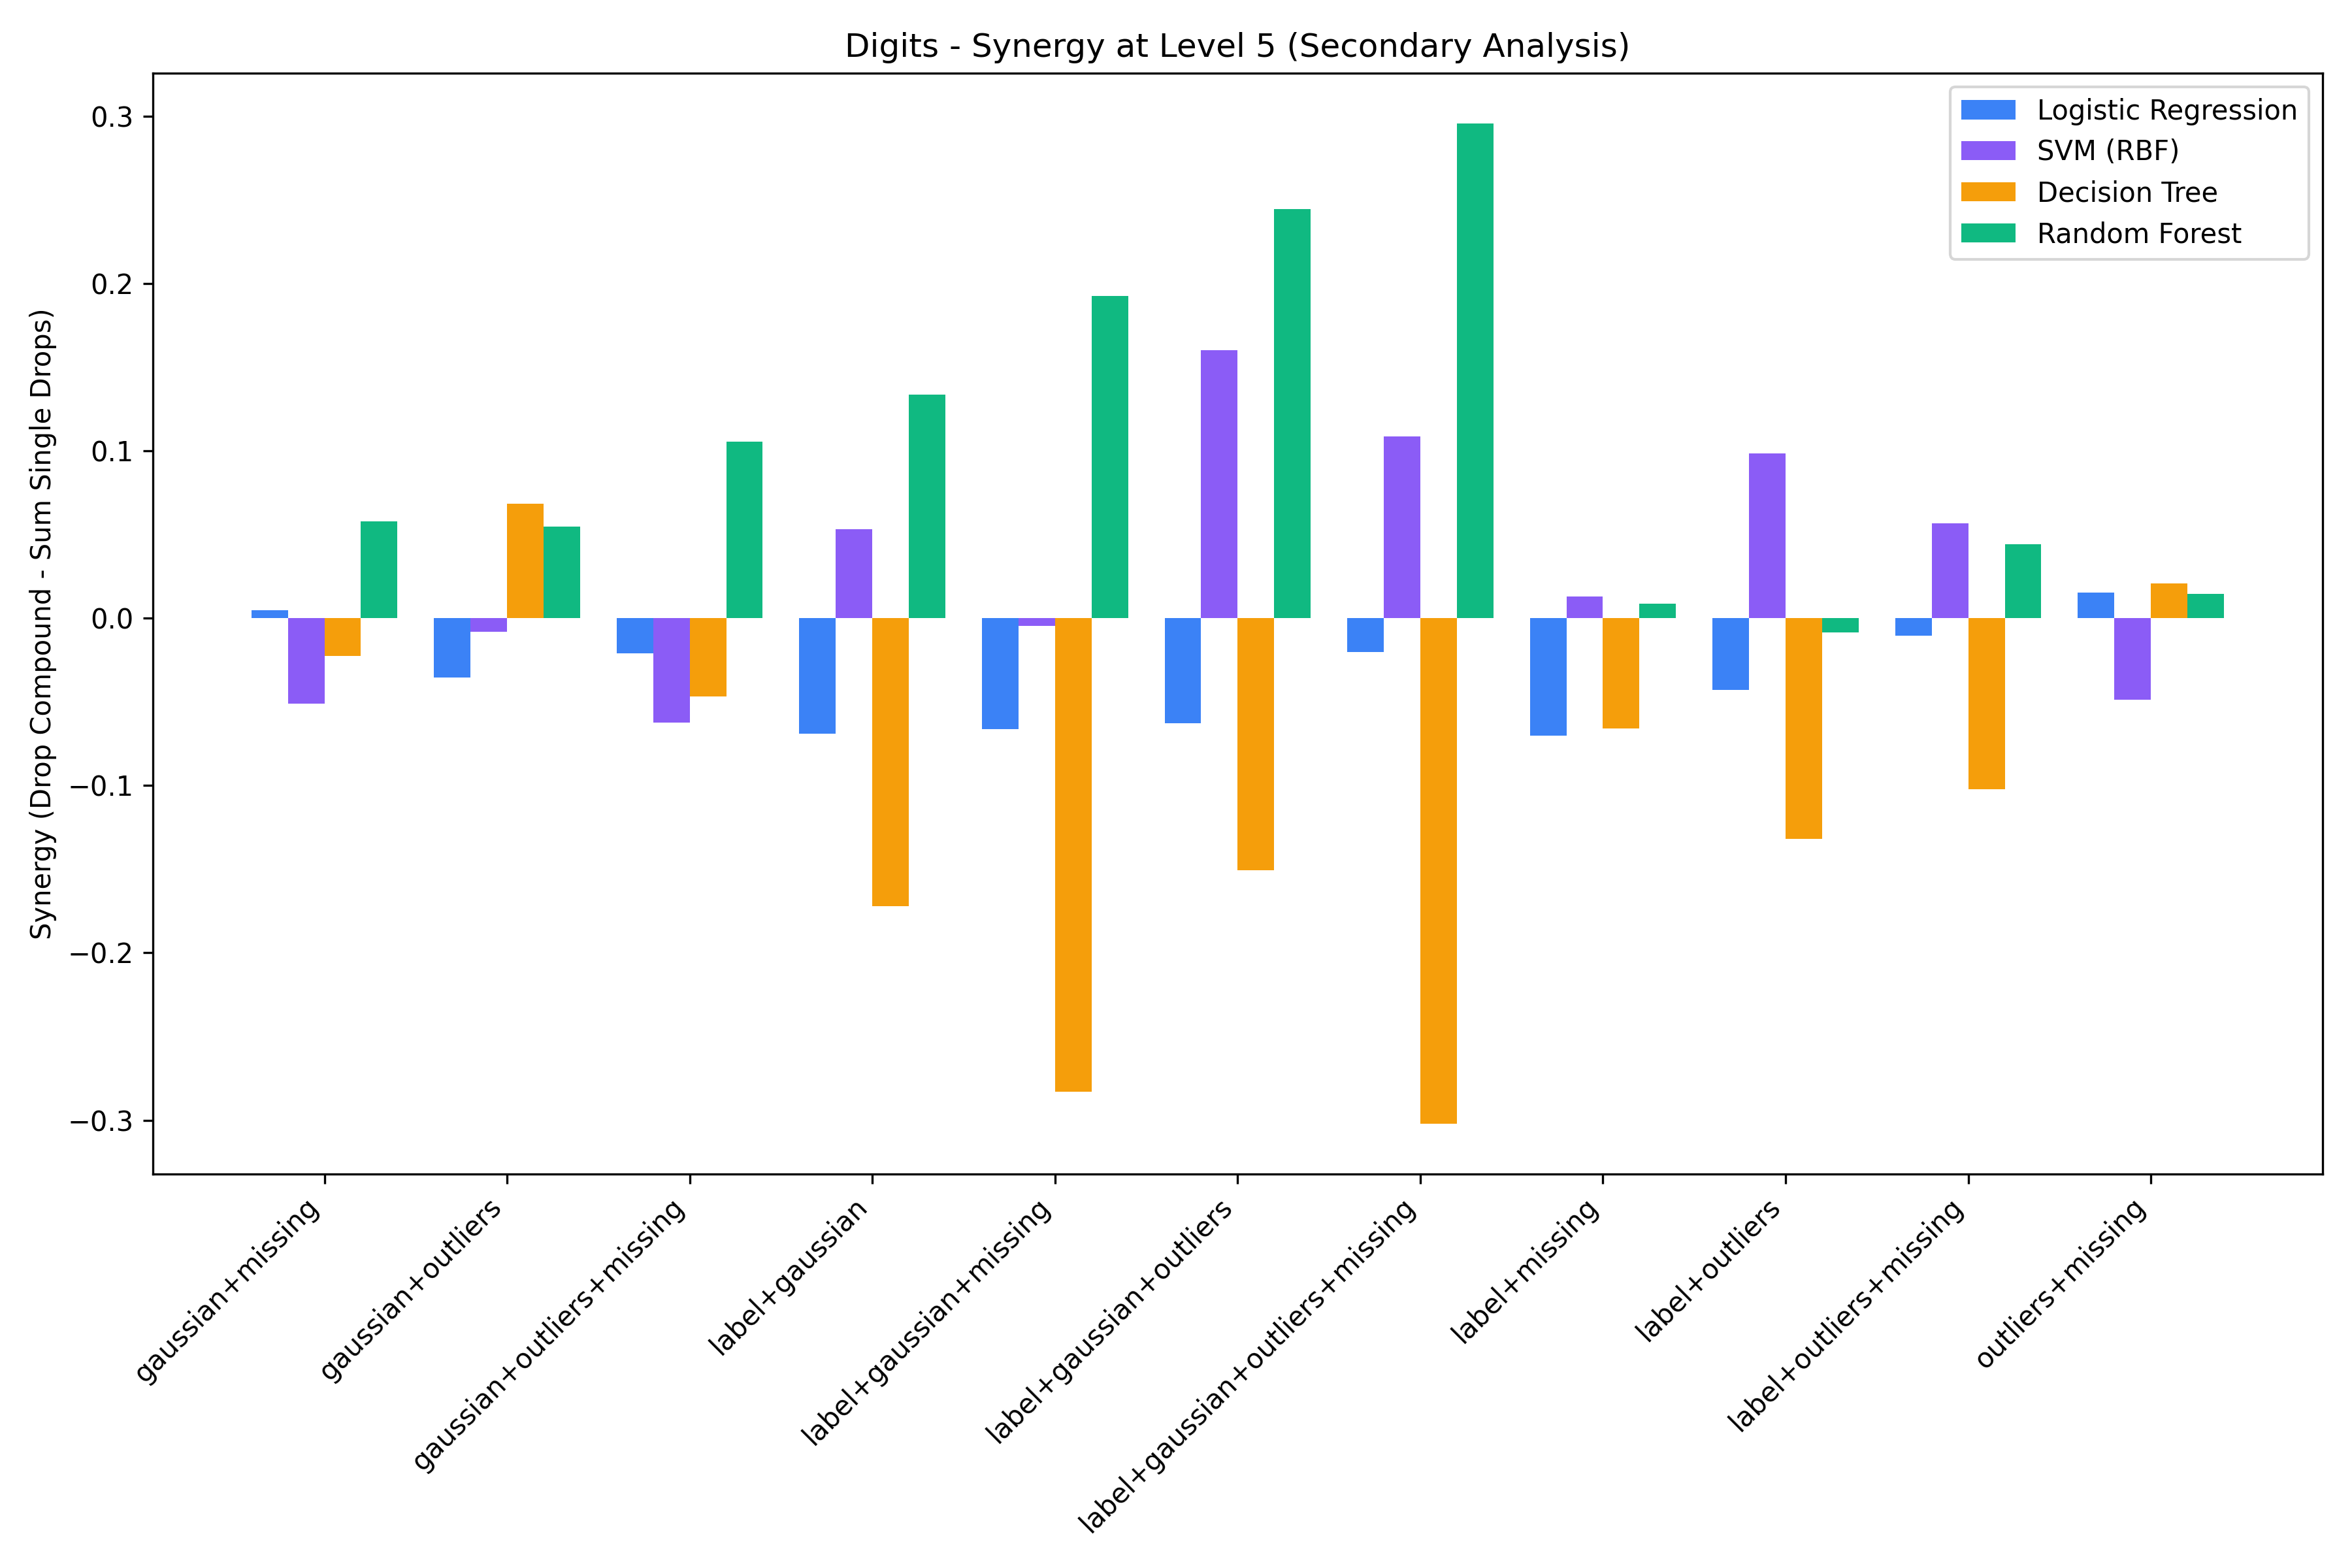
\includegraphics[width=0.95\textwidth]{figures/project_figures/digits-synergy.png}
\caption{Digits: synergy at level 5. The largest positive bars occur for high-severity combinations involving label and Gaussian noise.}
\label{fig:digits-syn}
\end{figure}

\section{Performance Analysis}

\subsection{Answers to the Research Questions}

\textbf{Q1: Which model is most robust overall?} There is no single winner on every measure. Random Forest has the highest mean BPI across the two datasets (5.100), while Logistic Regression has the highest mean RS (0.9423). On Breast Cancer, Logistic Regression is ranked first in the all-combination scope, and SVM is ranked first in the single-noise scope. On Digits, Random Forest is ranked first in both scopes. The Decision Tree is unambiguously the least robust model: it is last on both datasets, its BPI is 3.533 on average, and its RS is 0.8207. The practical answer therefore depends on the objective. If survival to a higher severity is the priority, Random Forest is the best overall choice. If retained performance across levels is the priority, Logistic Regression is marginally better. Both are preferable to the Decision Tree.

\textbf{Q2: Which noise type hurts most?} Label noise is the most damaging single corruption. Its mean breaking level is 4.375, compared with 5.250 for Gaussian noise, 5.625 for missing values, and 5.875 for outliers. Its mean level-5 Macro F1 drop is 0.1808, compared with 0.1251, 0.0531, and 0.0430 respectively. Label noise is also the only single corruption that breaks every model on Breast Cancer. Gaussian noise is the second most damaging corruption. Outliers and missing values are comparatively benign in isolation, but they can become harmful when combined with label noise or when they interact with other feature corruptions.

\textbf{Q3: What is each model's breaking point?} The complete single-noise breaking points are given in Table~\ref{tab:singlebp}, and the full set of 120 breaking points is visualised in Figures~\ref{fig:bc-heat} and~\ref{fig:digits-heat}. Of the 120 cells, 83 reached a breaking point and 37 did not. Breaking points are concentrated at levels 4 and 5 on Breast Cancer, but they are spread across levels 2--4 on Digits. The full per-combination table is written to the official results file.

\textbf{Q4: Is compound noise worse than the sum of single noises?} Compound noise is worse in absolute terms: the mean breaking level falls monotonically from 5.281 for single noise to 4.729 for pairs, 4.219 for triples, and 3.750 for the four-way combination. However, it is usually less than additive. Only 124 of 440 compound cells (28.2\%) have positive synergy. The mean synergy is negative on both datasets. Super-additive interactions do occur, especially on Digits at high severity, with the largest positive synergy (0.2958) for the Random Forest four-way combination at level 5. The answer is therefore nuanced: compound noise is more damaging than individual noise, but the sum of single-noise drops is usually an overestimate of the compound drop, except in a minority of high-severity multiclass cases where it is an underestimate.

\textbf{Q5: Do binary and multiclass data differ?} Yes, substantially. Digits is more fragile than Breast Cancer. The mean single-noise breaking level is 5.125 on Digits versus 5.438 on Breast Cancer; the mean compound breaking level is 3.864 versus 5.045; and the four-way breaking level is 2.750 versus 4.750. On Breast Cancer, 28 of the 36 reached breaking points occur at level 5, whereas on Digits only 10 of the 47 occur at level 5 and 19 occur at level 4. The multiclass dataset therefore fails earlier and more abruptly. Part of the difference is attributable to the task itself: a ten-class problem has more decision boundaries to corrupt, and Macro F1 penalises errors in small classes.

\subsection{Interpretation}

The dominance of label noise is consistent with the literature. A corrupted label directly contradicts the feature--label relationship that the model is trying to learn, and a flexible classifier can fit the corrupted examples rather than the underlying pattern \cite{zhang2021rethinking,song2023survey}. Gaussian feature noise is less direct: it perturbs the input but leaves the label unchanged, so a model can still recover the correct decision boundary if the perturbation is small relative to the class separation. Outliers and missing values are even less direct, especially because mean imputation and standardisation reduce their influence. This ordering is visible in the single-noise breaking points and in the level-5 drops.

The compound results show that corruption types are not independent. The four-way combination is the earliest-breaking setting on both datasets, and the three-way combinations that include label noise are consistently earlier than the pairs. The heatmaps make the pattern visible: the top rows, which contain label noise, are lighter than the rows that contain only feature corruption.

The model ranking is also interpretable. The Decision Tree partitions the feature space greedily and is highly sensitive to individual splits, so a small number of corrupted labels or shifted features can change the tree structure and cause large errors. The Random Forest averages many trees and is therefore more stable, which explains its higher BPI. Logistic Regression is a smooth linear model and is relatively stable on this data, which explains its high RS. SVM with an RBF kernel is strong on the clean Digits baseline and on single-noise Digits, but its performance under compound noise is more variable, which places it third in the Digits all-combination ranking.

The synergy results refine the ``compound noise is worse than the sum'' intuition. In most cells, the single-noise drops overlap: a cell that is already corrupted by label noise has less additional room to be damaged by missing values, so the compound drop is smaller than the sum. This produces negative synergy. In a small number of high-severity multiclass cells, the corruptions reinforce each other: label noise changes the target, Gaussian noise blurs the class boundary, and outliers or missing values shift the preprocessing statistics. The result is a compound drop that exceeds the sum, which produces positive synergy. The two Decision Tree floor-effect cases are an extreme version of this phenomenon, where the sum of single drops exceeds the baseline and the synergy interpretation becomes unstable.

\subsection{Comparison with Existing Methods}

Table~\ref{tab:litresults} compares the present findings with the core reviewed papers. The comparison is methodological rather than numerical, because the datasets, models, and noise models differ.

\begin{table}[H]
\centering
\caption{Comparison of the present findings with the reviewed literature.}
\label{tab:litresults}
\footnotesize
\begin{tabular}{p{1.7cm}p{2.3cm}p{2.7cm}p{3.0cm}p{2.7cm}}
\toprule
\textbf{Study} & \textbf{Focus} & \textbf{Setting} & \textbf{Main finding} & \textbf{Relation to this work} \\
\midrule
Song et al.\ \cite{song2023survey} & Label-noise-robust deep learning & 62 DNN methods; image benchmarks & Five-family taxonomy; no method satisfies all six properties & Provides the taxonomy; this work extends the question to classical tabular models and compound noise \\
Zhang et al.\ \cite{zhang2020hybrid} & Hybrid noise in multilabel learning & Feature and label noise; multilabel framework & Feature and label noise should be handled jointly & Motivates compound noise; this work uses single-label tabular data and breaking points \\
Zeng et al.\ \cite{zeng2025feature} & Feature noise as mitigation & Gaussian feature noise; deep networks; four datasets & Feature noise tightens the PAC-Bayes bound and improves accuracy under label noise & Confirms feature--label interaction; this work measures Gaussian noise as a corruption rather than a remedy \\
Chen \cite{chen2023compound} & Robust learning under compound noise & Outliers and noisy labels; semisupervised deep generative model & Compound noise requires dedicated robust modelling & Confirms that compound noise is a distinct problem; this work adds a systematic 15-combination sweep \\
\textbf{This work} & Breaking points under compound noise & Four classical models; two tabular datasets; 15 combinations, 5 levels, 10 seeds & Label noise is most damaging; compound noise lowers the breaking level; Digits is more fragile; Decision Tree is least robust & Complements the deep-learning literature with a reproducible classical tabular benchmark \\
\bottomrule
\end{tabular}
\end{table}

The findings agree with the literature on the central point that label noise is more harmful than input noise \cite{song2023survey}. They also support the observation that feature noise and label noise interact \cite{zeng2025feature}: Gaussian noise is the second most damaging single corruption, and the label + Gaussian combinations are among the earliest-breaking pairs. The compound-noise literature \cite{zhang2020hybrid,chen2023compound} is supported by the monotonic decrease in the breaking level as more noise types are combined.

The present work adds three things that are not available in the reviewed papers. First, it provides a complete fifteen-combination sweep on classical tabular models. Second, it reports a breaking point for every model and combination, rather than a single average score. Third, it decomposes the compound effect into single-noise and interaction components and shows that the interaction is usually negative but can be positive at high severity. These additions are complementary to the deep-learning literature, not a replacement for it.

\section{Discussion}

\subsection{Threats to Validity}

The results are subject to several limitations.

\begin{itemize}
  \item \textbf{Synthetic noise.} The four noise types are generated by controlled injectors. Real-world corruption may be instance-dependent, correlated across features, or structured in ways that the injectors do not capture. In particular, label noise is symmetric and class-independent, whereas real annotator errors are often class-dependent.
  \item \textbf{Two datasets.} Breast Cancer and Digits are small, well-studied tabular datasets. The findings may not generalise to larger, higher-dimensional, or heavily imbalanced tabular data.
  \item \textbf{Four classical models.} The conclusions apply to the four models and fixed hyperparameters used here. Hyperparameter tuning could change the absolute performance and, in principle, the ranking.
  \item \textbf{Threshold choice.} The breaking point uses a 90\% threshold. A different threshold would move the breaking points, although the ordering of the mean levels would be expected to remain similar.
  \item \textbf{Severity calibration.} The levels were calibrated on the MVP results and then frozen. Equal level numbers do not imply equal harm across noise types, and a different level table could change the absolute breaking levels.
  \item \textbf{Statistical inference.} The results are descriptive. Ten seeds provide a measure of variability, but no formal significance test or confidence interval is reported for the model rankings. The BPI and RS differences between adjacent models should therefore be interpreted with caution.
  \item \textbf{No mitigation.} The project measures degradation, not the effectiveness of mitigation. Robust losses, cleaning, or sample selection could improve the absolute results.
  \item \textbf{Clean test set.} The test set is clean by design, which isolates the effect of training-data corruption. It does not measure the effect of corrupted test data at inference time.
\end{itemize}

\subsection{Implications}

For practitioners working with classical models on tabular data, the results suggest a clear priority order. Label quality should be protected first, because label noise causes the earliest and largest degradation. Feature noise is the next priority, especially for tree-based models. Missing values and outliers are less damaging in isolation, but they should not be ignored in a compound-noise setting, because they can interact with label and Gaussian noise.

The choice of model should depend on the objective. Random Forest is a reasonable default when the goal is to survive to higher severity levels, and Logistic Regression is a reasonable default when the goal is to retain a high fraction of baseline performance. The Decision Tree should be used with caution in noisy settings, because it fails earlier and loses more performance than the other three models.

The compound results argue against relying on a single-noise robustness test. A model that looks robust under label noise alone may still fail when label noise is combined with feature noise or missing values. A compound test is therefore more informative than a single-corruption test, even when the individual corruptions are the same.

\section{Summary}

This chapter reported the frozen official results. The clean baselines, single-noise breaking points, compound-noise breaking levels, robustness rankings, and synergy analysis were presented with the corresponding figures. Label noise was the most damaging single corruption, compound noise was consistently more harmful than individual noise, and the multiclass dataset was more fragile than the binary dataset. The Decision Tree was the least robust model, while Random Forest and Logistic Regression led on different aggregate measures. Synergy was usually sub-additive but showed important super-additive exceptions at high severity on Digits. The results were compared with the reviewed literature, and the main threats to validity were discussed.

\chapter{Conclusion and Future Scope}

\section{Conclusion}

This project set out to map the breaking point of classical machine learning models under individual and compound training-data noise. The work was motivated by a gap in the literature: robustness is usually studied one corruption type at a time, often with deep networks and a small number of noise rates, while many practical tabular problems are solved with classical models under several simultaneous data-quality problems.

The project addressed the gap with a reproducible experiment framework. Two public tabular datasets, four fixed classical classifiers, four deterministic noise injectors, all fifteen non-empty noise combinations, and five severity levels were evaluated. The official Full run contains 6,080 fits over ten seeds, with a stratified 70/30 split, a clean test set, and a frozen methodology. A breaking point was defined as the first level at which mean Macro F1 falls to 90\% or less of the clean baseline, and two aggregate measures, BPI and RS, were used to rank the models. A secondary synergy analysis decomposed the compound effect into single-noise and interaction components.

The main findings are as follows.

\begin{itemize}
  \item Label noise is the most damaging single corruption, with a mean breaking level of 4.375 and a mean level-5 Macro F1 drop of 0.1808. Gaussian noise is second, followed by missing values and outliers.
  \item Compound noise is consistently more harmful than individual noise. The mean breaking level falls from 5.281 for single noise to 4.729 for pairs, 4.219 for triples, and 3.750 for the four-way combination.
  \item The multiclass Digits dataset is more fragile than the binary Breast Cancer dataset. Its mean compound breaking level is 3.864 versus 5.045, and its four-way breaking level is 2.750 versus 4.750.
  \item The Decision Tree is the least robust model on both datasets, with a mean BPI of 3.533 and a mean RS of 0.8207. Random Forest has the highest mean BPI (5.100), and Logistic Regression has the highest mean RS (0.9423).
  \item Synergy is usually negative: only 124 of 440 compound cells are worse than additive. Super-additive interactions do occur, most notably for Random Forest on Digits with the four-way combination at level 5.
\end{itemize}

The project also delivered a working software artefact: a Python experiment engine, a FastAPI service, a React visualization application, and a provenance and checksum mechanism that makes the official results auditable. The objectives stated in Chapter~1 were therefore met. The project did not propose a new mitigation algorithm; its contribution is a measurement framework and an empirical map that complements the existing deep-learning literature \cite{song2023survey,zeng2025feature,zhang2020hybrid,chen2023compound}.

\section{Limitations}

The conclusions should be read in the light of the following limitations.

\begin{itemize}
  \item \textbf{Limited dataset coverage.} Only two small tabular datasets were used. The results may not extend to larger, higher-dimensional, imbalanced, or domain-specific data.
  \item \textbf{Classical models only.} The study covers four classical classifiers with fixed hyperparameters. Deep networks, gradient boosting, and tuned models may behave differently.
  \item \textbf{Synthetic and symmetric noise.} The noise injectors are controlled and deterministic. Real corruption is often instance-dependent, class-dependent, and correlated across features.
  \item \textbf{Threshold sensitivity.} The breaking point depends on the 90\% threshold. A different threshold would change the absolute breaking levels, although the main ordering is likely to remain.
  \item \textbf{Level calibration.} Equal severity levels are not equally harmful across noise types. The calibrated level table is a deliberate simplification, and a different table could shift the absolute results.
  \item \textbf{Descriptive analysis.} The results are summarised with means and standard deviations over ten seeds, but no formal hypothesis tests or confidence intervals are reported for the ranking differences.
  \item \textbf{No mitigation.} The project measures degradation rather than the effectiveness of cleaning, robust losses, or sample selection.
  \item \textbf{Clean test set.} The test set is clean by design, so the study does not measure the effect of corrupted data at inference time.
\end{itemize}

\section{Future Scope}

Several extensions would strengthen the work.

\begin{enumerate}
  \item \textbf{Deep and ensemble models.} Repeat the protocol with multilayer perceptrons, gradient-boosted trees, and other ensemble methods to test whether the breaking-point ordering is model-family dependent.
  \item \textbf{Additional datasets.} Add larger, imbalanced, and domain-specific tabular datasets, including medical, financial, and sensor data, to test the generality of the findings.
  \item \textbf{Real-world noise.} Replace or supplement synthetic noise with instance-dependent and class-dependent noise estimated from real annotation processes.
  \item \textbf{Additional noise types.} Study irrelevant features, duplicated features, feature scaling errors, and correlated missingness.
  \item \textbf{Mitigation experiments.} Apply robust losses, sample selection, cleaning, and imputation strategies at each severity level and measure how much they shift the breaking point.
  \item \textbf{Statistical inference.} Add confidence intervals, paired tests, and effect sizes for the model rankings and the synergy estimates.
  \item \textbf{Adaptive severity calibration.} Calibrate levels separately for each noise type so that equal levels correspond to comparable measured harm.
  \item \textbf{Deployment hardening.} Add authentication, role-based access control, HTTPS, rate limiting, and audit logging before exposing the API beyond a local environment.
\end{enumerate}

\section{Final Remarks}

The phrase ``death by a thousand cuts'' is a useful description of compound data corruption. A single small defect may be tolerable, but several defects together can push a model past its breaking point. This project provides a reproducible way to locate that point for classical tabular models and shows that the combined effect is usually, but not always, less than additive. The framework, the frozen results, and the interactive application provide a foundation for further work on data quality and model robustness.


% =========================================================
% REFERENCES
% =========================================================
\clearpage
\addcontentsline{toc}{chapter}{References}
\bibliographystyle{IEEEtran}
\bibliography{references}

% =========================================================
% APPENDIX
% =========================================================
\clearpage
\appendix
\chapter{Appendix}
This appendix presents the open-source contribution and the Sustainable Development Goals associated with the project.

\section{Open Source Contribution}
\begin{itemize}[nosep]
\item \textbf{Project / Repository:} Lastbook
\item \textbf{Platform:} GitHub
\item \textbf{Student contributors:} Rushikesh Tathe, Nihar Gudekar, and Mohammad Ali Sayyed
\item \textbf{Nature of contribution:} Added a video playback-speed selector with options from 0.5$\times$ to 2$\times$, synchronised with the video. The change was tested in Microsoft Edge and with the project test suite.
\item \textbf{Pull request:} \#132, submitted and awaiting review.
\item \textbf{Repository:} \textcolor{blue}{\url{https://github.com/Immortal-Protocols/lastbook}}
\item \textbf{Pull request link:} \textcolor{blue}{\url{https://github.com/Immortal-Protocols/lastbook/pull/132}}
\end{itemize}
\subsection{Evidence}
The following screenshots show the contribution branch and its commit history.
\begin{figure}[H]
\centering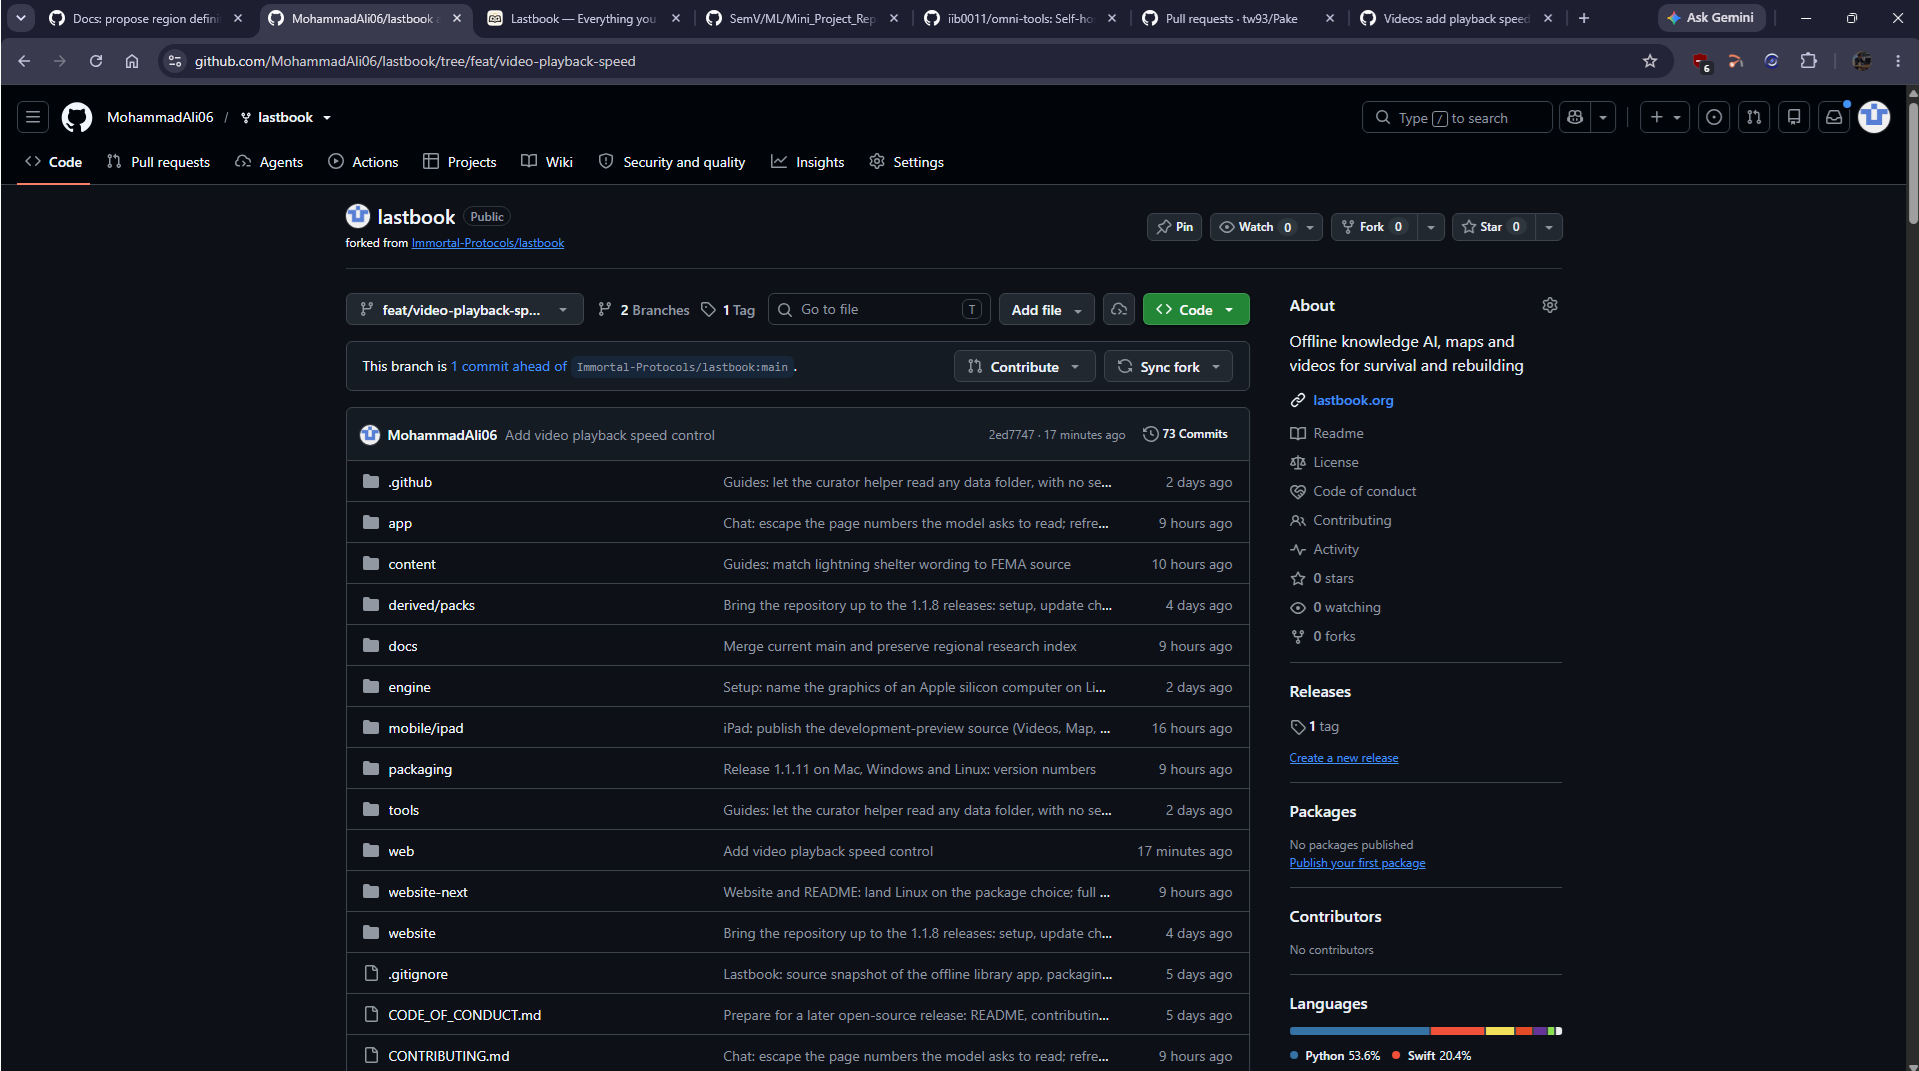
\includegraphics[width=0.96\textwidth,height=0.37\textheight,keepaspectratio]{figures/lastbook_pr.png}
\caption{Lastbook playback-speed contribution branch}
\end{figure}
\begin{figure}[H]
\centering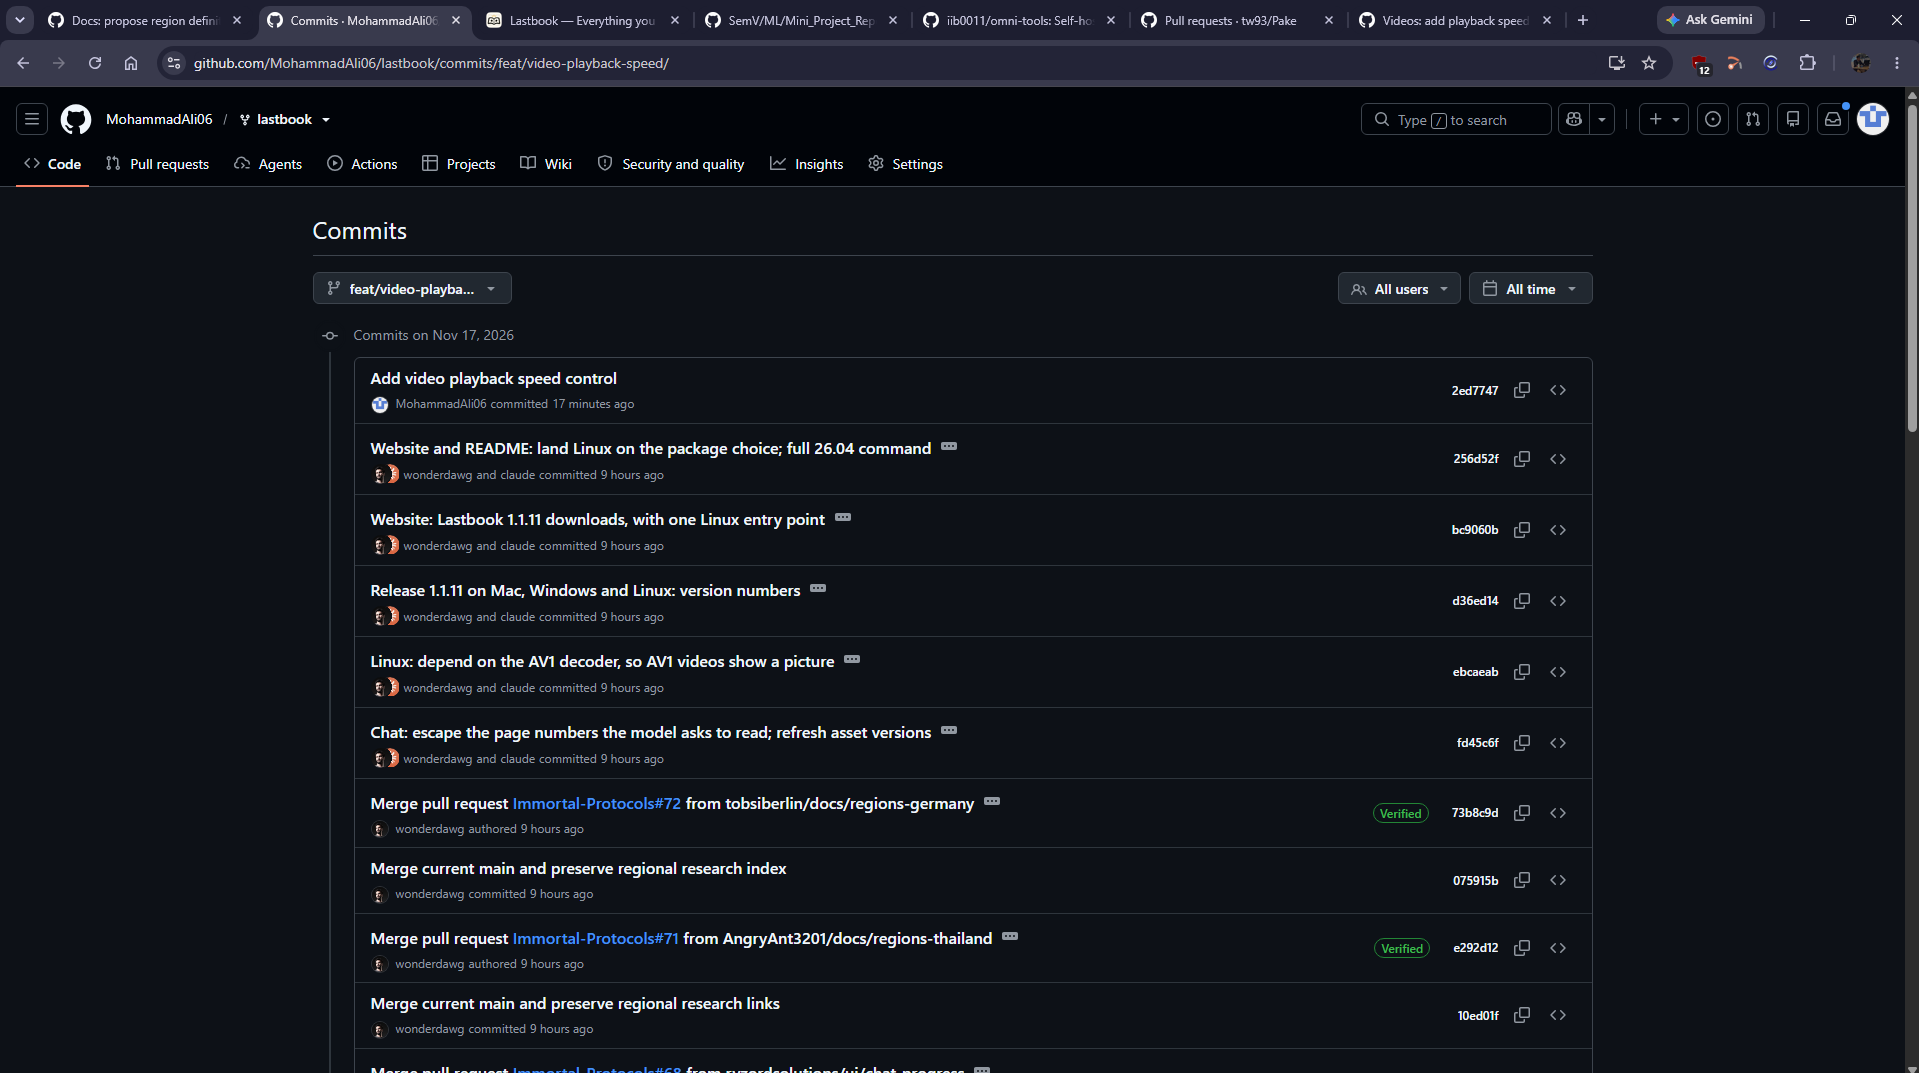
\includegraphics[width=0.96\textwidth,height=0.37\textheight,keepaspectratio]{figures/lastbook_commit.png}
\caption{Commit associated with the contribution}
\end{figure}
\section{SDG Goals Achieved}
The project and open-source contribution indirectly support the following goals:
\begin{itemize}
\item \textbf{SDG 3 -- Good Health and Well-being:} Analysing model robustness on a medical dataset encourages attention to data quality in health-related decision support.
\item \textbf{SDG 4 -- Quality Education:} The reproducible benchmark supports learning about data quality and machine-learning evaluation; adjustable playback speed can help viewers learn at their preferred pace.
\item \textbf{SDG 9 -- Industry, Innovation and Infrastructure:} Reproducible experiment tooling and the open-source software contribution support accessible, reusable digital infrastructure.
\end{itemize}



\end{document}
